%% 
%% Copyright 2007-2024 Elsevier Ltd
%% 
%% This file is part of the 'Elsarticle Bundle'.
%% ---------------------------------------------
%% 
%% It may be distributed under the conditions of the LaTeX Project Public
%% License, either version 1.3 of this license or (at your option) any
%% later version.  The latest version of this license is in
%%    http://www.latex-project.org/lppl.txt
%% and version 1.3 or later is part of all distributions of LaTeX
%% version 1999/12/01 or later.
%% 
%% The list of all files belonging to the 'Elsarticle Bundle' is
%% given in the file `manifest.txt'.
%% 
%% Template article for Elsevier's document class `elsarticle'
%% with harvard style bibliographic references

%\documentclass[review,3p,authoryear]{elsarticle}

%% Use the option review to obtain double line spacing
%%\documentclass[authoryear,preprint,review,12pt]{elsarticle}

%% Use the options 1p,twocolumn; 3p; 3p,twocolumn; 5p; or 5p,twocolumn
%% for a journal layout:
%% \documentclass[final,1p,times,authoryear]{elsarticle}
%% \documentclass[final,1p,times,twocolumn,authoryear]{elsarticle}
\documentclass[final,3p,times,authoryear]{elsarticle}
%% \documentclass[final,3p,times,twocolumn,authoryear]{elsarticle}
%% \documentclass[final,5p,times,authoryear]{elsarticle}
%% \documentclass[final,5p,times,twocolumn,authoryear]{elsarticle}

%% For including figures, graphicx.sty has been loaded in
%% elsarticle.cls. If you prefer to use the old commands
%% please give \usepackage{epsfig}

%% The amssymb package provides various useful mathematical symbols
\usepackage{amssymb}
%% The amsmath package provides various useful equation environments.
\usepackage{amsmath}
%% The amsthm package provides extended theorem environments
%% \usepackage{amsthm}

%% Commands for TODO notes
\usepackage{xargs}                      % Use more than one optional parameter in a new commands
\usepackage[pdftex,dvipsnames]{xcolor}  % Coloured text etc.
\usepackage[colorinlistoftodos,prependcaption,textsize=tiny]{todonotes}
\newcommandx{\unsure}[2][1=]{\todo[linecolor=red,backgroundcolor=red!25,bordercolor=red,#1]{#2}}
\newcommandx{\change}[2][1=]{\todo[linecolor=blue,backgroundcolor=blue!25,bordercolor=blue,#1]{#2}}
\newcommandx{\info}[2][1=]{\todo[linecolor=OliveGreen,backgroundcolor=OliveGreen!25,bordercolor=OliveGreen,#1]{#2}}
\newcommandx{\improvement}[2][1=]{\todo[linecolor=Plum,backgroundcolor=Plum!25,bordercolor=Plum,#1]{#2}}


\usepackage{amssymb}

%% The line no packages add line numbers. Start line numbering with
%% \begin{linenumbers}, end it with \end{linenumbers}. Or switch it on
%% for the whole article with \linenumbers.
% \usepackage{lineno}
\usepackage{amssymb,amsthm}
\usepackage{optidef}
\usepackage{multirow}
\usepackage[normalem]{ulem}
\useunder{\uline}{\ul}{}
\usepackage{hyperref}
\usepackage{placeins}
\newtheorem{defn}{Definition}
\newtheorem{lemma}{Lemma}
\newtheorem{prop}{Proposition}
\newtheorem{ex}{Example}
\newtheorem{hypo}{Hypothesis}
\newtheorem{theo}{Theorem}
% \usepackage[ruled,vlined,linesnumbered]{algorithm2e}
%% The amsthm package provides extended theorem environments
%% \usepackage{amsthm}

\usepackage{booktabs}
\def\1{{1\kern-.3468em{ 1}}}

%\usepackage{graphicx, color, soul}
\usepackage{xcolor}

%% tabelas mais bonitas
\usepackage{booktabs}

% Para adicionar espaços após comandos
\usepackage{xspace}

\usepackage{subcaption}

\usepackage{amsfonts, amsmath, amssymb, mathtools, latexsym, bbm}

% Teoremas, definições, proposições, lemas, corolários e conjecturas
% Pode dar conflito com outros pacotes
\usepackage{amsthm}

\newcommand{\hcunicamp}{HC - Unicamp}
% \newcommand{\rqpolicy}{\(R,Q\)}
\newcommand{\rqmodule}{Queue-management module}
\newcommand{\overtimemodule}{Overtime and cancellation module}
\newcommand{\preprocessmodule}{Preprocessing of strategic input / block-demand conversion}
\newcommand{\otschedmodule}{Operating theatre scheduling module}


% ==================================================
% Queue-management module
% ==================================================

\newcommand{\rthreshold}{R}
\newcommand{\batchsizeq}{Q}
\newcommand{\lowq}{\underline{\batchsizeq}} % lower bound on Q in number of patients
\newcommand{\upq}{\overline{\batchsizeq}} % upper bound on Q in number of patients
\newcommand{\conflevel}{\alpha}
\newcommand{\waittimereq}{\tau}

\newcommand{\stocprocperiod}{t}
\newcommand{\stocprocqueue}[1]{X_{#1}}
\newcommand{\stocprocbatches}[1]{Y_{#1}}
\newcommand{\stocprocremain}[1]{Z_{#1}}
\newcommand{\stocprocremainstate}{z}

\newcommand{\rvdemand}{D}
\newcommand{\drawnrvdemand}{d}
\newcommand{\roundbatches}{A}
\newcommand{\maxnumberbatch}{M}

\newcommand{\statespace}{S}

\newcommand{\steadystate}[1]{\pi_{#1}}
\newcommand{\transmatrix}[1]{P_{#1}}
\newcommand{\transmatrixval}[2]{p_{#1}^{#2}}

% ==================================================
% Overtime and cancellation module
% ==================================================

% indices
\newcommand{\surgidx}{i}
\newcommand{\completedsurgsidx}{k}
% \newcommand{\cancellationsidx}{u}

% parameters
\newcommand{\blocklength}{T}
\newcommand{\safetythreshold}{t^{*}}
\newcommand{\probstoppingthreshold}{\varepsilon_{\text{stop}}}
\newcommand{\plannedsurgs}{n}
\newcommand{\optplannedsurgs}{n^*}
\newcommand{\durationpmf}{p}
\newcommand{\excesscost}{c}
\newcommand{\overtimepenalty}{p}
\newcommand{\cancelledsurgeries}{\ell}

% random variables
\newcommand{\rvsurgdur}{T_D}

\newcommand{\duration}{d}
\newcommand{\cumulativeduration}[1]{s_{#1}}
\newcommand{\numcompletedsurgs}{K}

% functions
% \newcommand{\cumulativedurationcdf}{F_{s_k}}
\newcommand{\convolve}{\text{Convolve}}
\newcommand{\calccdf}{\text{CalculateCDF}}
\newcommand{\runnewsvendor}{\text{RunNewsvendor}}
\newcommand{\gain}[1]{G(#1)}
\newcommand{\cancellationcost}{C}
\newcommand{\netvalue}{\Delta}
\newcommand{\marginalvalue}{g}
\newcommand{\cancellationfunction}{cost}

% auxiliary algorithm output
\newcommand{\survivalvector}{q}

% ==================================================
% Preprocessing of strategic input / block-demand conversion
% ==================================================

% parameters
\newcommand{\blocksurgpmf}{p}
\newcommand{\targetq}{{Q'}}

% index for successive convolutions / number of aggregated blocks
\newcommand{\convidx}{counter}
\newcommand{\convnumber}{n}

% random variable
% \newcommand{\totalsurgs}{S}

% outputs in block units
\newcommand{\blockdemand}{B}
\newcommand{\lowerblockdemand}{\underline{\blockdemand}_{\specialtyidx}}
\newcommand{\upperblockdemand}{\overline{\blockdemand}_{\specialtyidx}}


% ==================================================
% MILP Sets and indices
% ==================================================

\newcommand{\blockset}{\mathcal{B}}
\newcommand{\blockmset}{\mathcal{B'}}
\newcommand{\blockidx}{b}
\newcommand{\blocki}{b_i}
\newcommand{\blockj}{b_j}

\newcommand{\roomset}{OT}
\newcommand{\roomsete}{\roomset_{e}}
\newcommand{\roomseta}{\roomset_{a}}
\newcommand{\roomidx}{ot}
\newcommand{\roomidxalt}{ot'}

\newcommand{\specialtyset}{Spec}
\newcommand{\specialtymset}{\specialtyset_{seq}}   % especialidades que precisam de dois blocos
\newcommand{\specialtycset}{\specialtyset_{circ}}  % especialidades circunstanciais
\newcommand{\specialtyprset}{\specialtyset_{prio}} % especialidades prioritárias
\newcommand{\specialtytxset}{\specialtyset_{tx}}% especialidades de transplante
\newcommand{\specialtyidx}{s}

\newcommand{\planninghorizonset}{D}
\newcommand{\planninghorizonidx}{d}

\newcommand{\timeperiodset}{M}
\newcommand{\timeperiodidx}{m}

% ==================================================
% MILP Decision variables
% ==================================================

\newcommand{\blockvar}{x_{\roomidx\blockidx\specialtyidx}}
\newcommand{\blockivar}{x_{\roomidx\blocki\specialtyidx}}
\newcommand{\blockjvar}{x_{\roomidx\blockj\specialtyidx}}
\newcommand{\deficitvar}{z_{\specialtyidx}}
\newcommand{\precvar}{y_{\roomidx\planninghorizonidx\specialtyidx}}
\newcommand{\integervar}{w_{\blockidx\specialtyidx}}
% \newcommand{\balancevar}{L}
\newcommand{\teamslackvar}{z_{\specialtyidx\blockidx}}
\newcommand{\anestslackvar}{a_{\blockidx}}

% ==================================================
% MILP parameters
% ==================================================

% \newcommand{\roomtospecialty}{\psi}
% \newcommand{\demand}{\delta}
% \newcommand{\numbersurgeons}{NumSurgeons}
\newcommand{\numbersanests}{NumAnests}
\newcommand{\needanest}{NeedAnest}
\newcommand{\specteams}{NumTeams}
% \newcommand{\mindeficit}{\beta}
\newcommand{\days}{|\planninghorizonset|}
\newcommand{\eps}{\epsilon}
\newcommand{\allowedrooms}{\lambda}
\newcommand{\entiredayroom}{EntireDayRoom}
\newcommand{\anestconstant}{\gamma}

\newcommand{\modelname}{OTScheduling}

% para pseudocódigo
\usepackage{algorithm}
% \usepackage{algorithmic}
\usepackage{algpseudocode}

\usepackage{tikz}
\usetikzlibrary{arrows.meta, positioning, fit, calc, shapes.symbols}

%% The lineno packages adds line numbers. Start line numbering with
%% \begin{linenumbers}, end it with \end{linenumbers}. Or switch it on
%% for the whole article with \linenumbers.
%% \usepackage{lineno}

\journal{European Journal of Operational Research}

\setlength {\marginparwidth}{2cm} % para os TODOs
\begin{document}

\begin{frontmatter}

%% Title, authors and addresses

%% use the tnoteref command within \title for footnotes;
%% use the tnotetext command for theassociated footnote;
%% use the fnref command within \author or \affiliation for footnotes;
%% use the fntext command for theassociated footnote;
%% use the corref command within \author for corresponding author footnotes;
%% use the cortext command for theassociated footnote;
%% use the ead command for the email address,
%% and the form \ead[url] for the home page:
%% \title{Title\tnoteref{label1}}
%% \tnotetext[label1]{}
%% \author{Name\corref{cor1}\fnref{label2}}
%% \ead{email address}
%% \ead[url]{home page}
%% \fntext[label2]{}
%% \cortext[cor1]{}
%% \affiliation{organization={},
%%            addressline={}, 
%%            city={},
%%            postcode={}, 
%%            state={},
%%            country={}}
%% \fntext[label3]{}

\title{Modular Framework for Long-term Surgery Planning Management under Uncertainty: From Strategic to Tactical Planning} %% Article title

%% use optional labels to link authors explicitly to addresses:
%% \author[label1,label2]{}
%% \affiliation[label1]{organization={},
%%             addressline={},

%%             city={},
%%             postcode={},
%%             state={},
%%             country={}}
%%
%% \affiliation[label2]{organization={},
%%             addressline={},
%%             city={},
%%             postcode={},
%%             state={},
%%             country={}}

\author[1]{João P. F. da Silva} \ead{joao.silva@ic.unicamp.br} %% Author name
\author[1]{Lucas Bortoletto} \ead{l173422@dac.unicamp.br}
\author[1]{Rafael C. S. Schouery} \ead{rcss@unicamp.br}
\author[2]{Edilson F. Arruda \corref{cor1}} \ead{e.f.arruda@southampton.ac.uk}

\cortext[cor1]{Corresponding author. Tel.: (+44)(0)2380 597146.}

%% Author affiliation
\affiliation[1]{organization={Institute of Computing, University of Campinas},%Department and Organization
            addressline={}, 
            city={Campinas},
            postcode={13083–852}, 
            state={SP},
            country={Brazil}}

\affiliation[2]{organization={Centre for Healthcare Analytics, Southampton Business School, University of Southampton},%Department and Organization
            addressline={}, 
            city={Southampton},
            postcode={}, 
            state={},
            country={UK}}



%% Abstract
\begin{abstract}
%% Text of abstract
Abstract text.
\end{abstract}

%%Graphical abstract
% \begin{graphicalabstract}
%     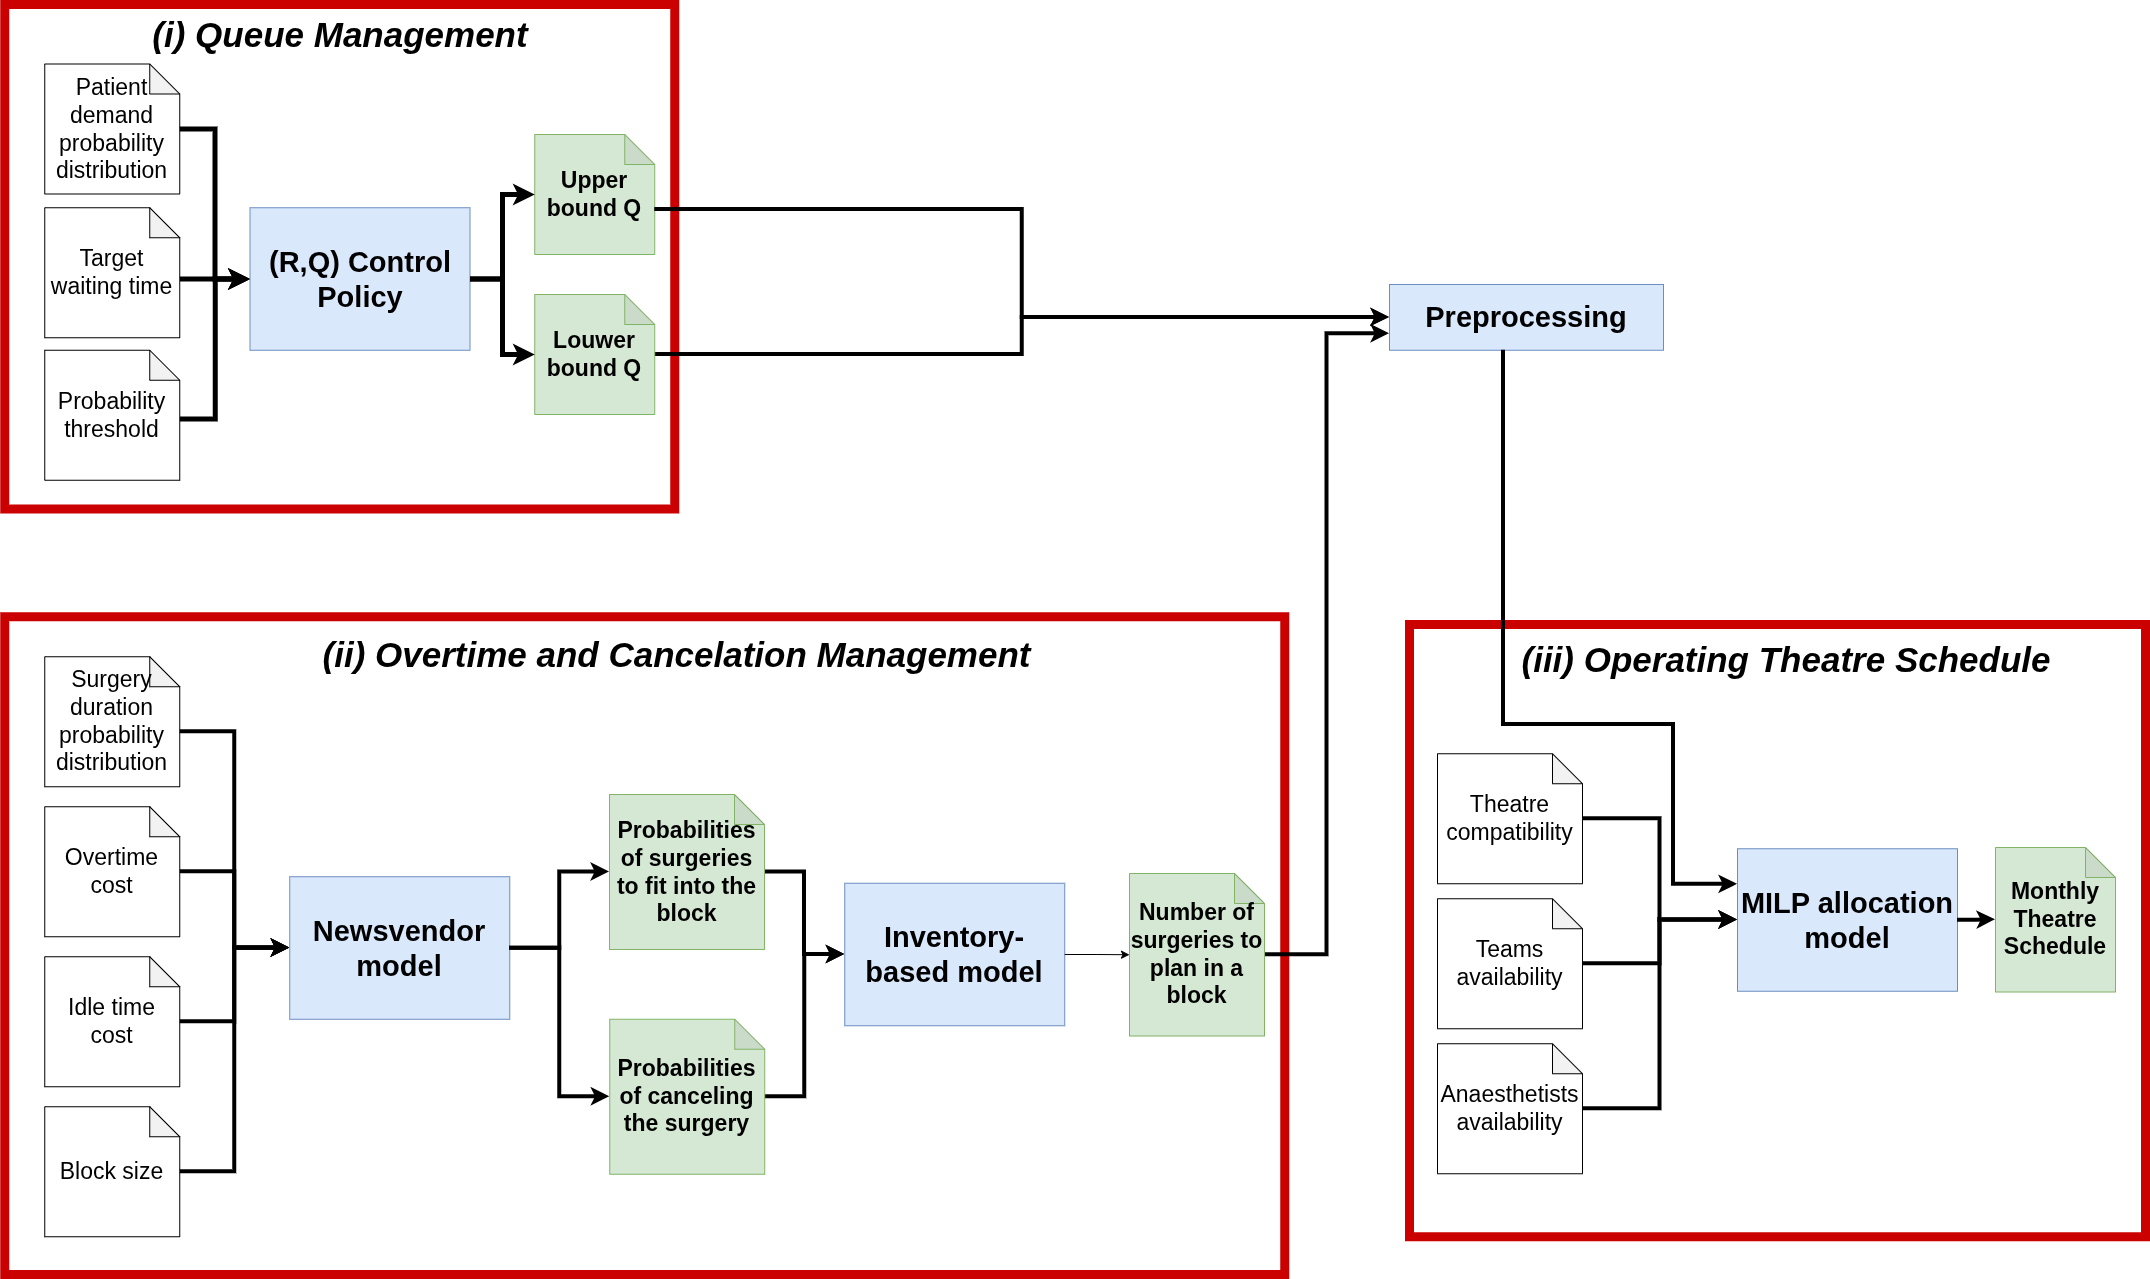
\includegraphics[width=0.8\textwidth]{images/diagram.png}
% \end{graphicalabstract}

%%Research highlights
% \begin{highlights}
% \item Research highlight 1
% \item Research highlight 2
% \end{highlights}

%% Keywords
\begin{keyword}
%% keywords here, in the form: keyword \sep keyword

%% PACS codes here, in the form: \PACS code \sep code

%% MSC codes here, in the form: \MSC code \sep code
%% or \MSC[2008] code \sep code (2000 is the default)

\end{keyword}

\end{frontmatter}

% \include{intro}

% ********************************************* %
\section{Related Works\label{sec:lit_review}}
% ********************************************* %

Surgery scheduling problems have traditionally been classified into three planning levels with different sources of uncertainty: strategic, tactical, and operational~\citep{Rahimi2020Review, Cardoen2010, wang2021operating, Melo2025}. 
At the strategic level, long-term decisions define the desired split of the capacity into specific surgical specialities and specify patient volumes of different medical specialties to be admitted over the planning horizon~\citep{Burdett2023} --- a process commonly referred to as Case Mix Planning (CMP).
Different objectives have been introduced at this level, such as maximizing profit~\citep{Fugener2015, Ma2013Mult} or minimizing long-term costs~\citep{Hof2015Casemix, Mcrae2020}. 
The tactical level defines a cyclic schedule (often weekly) commonly known as Master Surgery Schedule (MSS)~\citep{Bovim2020,Siqueira2018INTO,Carneiro2025}. 
The MSS step allocates time blocks in operating theatres to surgical teams and is reviewed in a medium-term horizon (e.g., monthly or quarterly). 
Finally, the operational level focuses on the daily operation and derives a Surgical Case Schedule (SCS), which generally assigns individual patients to time blocks previously allocated to specific surgical teams at the tactical level~\citep{Vieira2025, Harris2022}.

Despite the large body of literature in surgery scheduling, there are significant gaps to be bridged. For example, inter-level integration remains limited in scope, often focusing on short-term alignment between surgeries and post-surgical bed occupation, and generally relying on deterministic approaches~\citep{Melo2025,wang2021operating, Siqueira2018INTO}. 
Furthermore, regardless of the planning level, strategies with a focus on guaranteeing waiting time requirements for patients still remain to be proposed. 
This is probably due to the complex propagation of uncertainty over different planning levels, which demands hybrid approaches that combine mathematical programming, stochastic modelling and queuing theory. %It is this gap that this paper will address.

% 2 - Na literatura, como tratam o Case Mix integrado ao Master Schedule? Consideram incerteza na demanda? Se sim, qual o impacto e qual a limitação?
The inherent interconnection between the strategic and tactical levels has motivated unified frameworks that link CMP and MSS decisions~\citep{Melo2025}. 
These often adopt sequential or joint optimisation approaches where case mix decisions act as the input to surgery scheduling models \citep{Ma2013Mult, Fugener2015}.
Modelling approaches typically consist of Mixed Integer Programming (MIP) formulations that focus on maximising hospital profit subject to Operating Theatre (OT) and bed capacity constraints.
While these frameworks acknowledge uncertainty, it is generally confined to downstream elements such as length of stay or ward occupancy.
Although modelling post-surgical congestion is relevant, such partial treatments remain short-sighted when not complemented by uncertainty in surgery durations and, crucially, by an explicit modelling of dynamic waiting lists across surgical specialities, which constitute the starting point of the entire planning process.

The perspective can be broadened by incorporating additional uncertainty sources and dynamic elements.
For instance,~\citet{Liu2019} model elective admissions through a Markov Decision Process (MDP), highlighting the role of waiting-list size in guiding strategic decisions.
Despite its conceptual value, the framework disregards essential practical constraints, such as surgeon availability, block scheduling and case-mix heterogeneity, thereby limiting practical applicability.
Similarly,~\citet{Mcrae2020} demonstrate that explicitly modelling uncertainty and selecting appropriate aggregation levels can significantly improve CMP outcomes and enable joint CMP-MSS optimisation.
Nevertheless, waiting-list dynamics remain outside of the modelling scope, implying no full integration of strategic and tactical decisions. 
Furthermore, their reliance on Sample Average Approximation (SAA) leads to representations that may understate distributional variability. 
%Taken together, 
These studies underscore the value of integrating CMP and MSS, yet they also reveal persistent shortcomings: uncertainty is represented only selectively across planning levels, waiting-list requirements are rarely modelled explicitly, and key operational constraints required for real-world implementation remain overlooked.

% 3 - Na literatura, como consideram cancelamento e overtime? Qual o impacto de considerar isso e até onde foram nesse sentido? (tentar não fugir de problemas que integram CM e MSS)
Uncertainty in surgery duration is another important issue that, when disregarded, may result in unpredictable idle or overtime in operating theatres~\citep{shehadeh2022stochastic}. 
Whilst overtime is costly and can lead to  cancellations that compromise the quality of care, idle time reflects an inadequate use of operating theatre capacity~\citep{shehadeh2022stochastic, Harris2022, Kayvanfar2025}. 
% Works that explicitly consider overtime generally seek to maximise the use of the available operating hours whilst somehow mitigating the risk of overtime. 
With the aim of maximising hospital revenue while preventing excessive overtime, \citet{Barz2015} propose a tactical patient admission and scheduling problem that derives a CMP under multiple resource constraints and stochastic clinical progression. 
The approach utilises a newsvendor heuristic to reserve capacity for emergency arrivals, and an MDP model to select the patient cohort to be admitted whilst considering probabilistic transitions between clinical states. 
The model, however, excludes the possibility of cancellations or postponements driven by overtime, as it assumes that the hospital always disposes of the resources to treat each admitted patient. 
%The authors model patients' health evolution as a MDP, where each clinical state deterministically defines daily resource consumption, solve it via Approximate Dynamic Programming (ADP), complemented by a newsvendor-based heuristic to determine capacity reservations for emergency arrivals. 
%Their objective is to maximise hospital revenue by admitting high-contribution elective patients while preventing excessive overtime.
%However, once a patient is admitted, the hospital is assumed to always provide the required resources. 
%This assumption excludes the possibility of cancellations or postponements driven by overtime. 
Moreover, by treating resource consumption as deterministic, the framework effectively ignores uncertainty in surgery duration --- one of the main drivers of operational instability. 
As a result, the model underestimates the practical interplay between stochastic surgery durations, cancellations and overtime, limiting its applicability to integrated CMP-MSS decision-making.

Furthermore,~\citet{Zhang2020} study a tactical surgery planning with the explicit aim of mitigating overtime risk when allocating elective patients to OTs over an upcoming planning horizon. 
Their model accounts for stochastic surgery durations and adopts a risk-averse objective that jointly captures both the probability and the expected magnitude of overtime, extending earlier approaches that consider only one of these dimensions~\citep{Shylo2013, Rath2017}.
Although they derive the durations from real-world data, eventually they approximate it through a set of discrete scenarios, limiting the full distributional representation.
A similar treatment appears in~\citet{Shehadeh2026}, which introduces a Distributionally Robust Optimisation (DRO) approach to address uncertainty in surgery durations.
While their approach minimises worst-case expected cost over an ambiguity set defined by known moments and support, it likewise relies on scenario-based representations.
Accurately capturing surgery-duration variability requires a large number of scenarios, substantially increasing computational burden and potentially undermining the practical advantages of DRO and related methods.

These limitations regarding the integration of overtime management and its associated cancellation risks into surgical planning frameworks highlight important research gaps.
There remains a need for models that explicitly incorporate cancellation dynamics induced by overtime and that provide a more thorough representation of surgery-duration uncertainty beyond scenario-based approximations. A key challenge which we tackle in this paper is to develop a modular approach to capture full distributional characteristics to build a planning model and use its output to feed an integrated CMP-MSS approach --- i.e., not solving an entire model at once.
%It is rather possible to capture full distributional characteristics to build a planning model and use its output to feed an integrated CMP-MSS approach --- i.e., not solving an entire model at once.

An additional and often underexplored dimension in integrated surgical planning concerns the incorporation of practical constraints inherent to real-world healthcare settings. 
Certain surgical activities, such as organ transplantation, impose rigid scheduling requirements that are difficult to reconcile with standard optimisation assumptions~\citep{Silva2025}. 
Furthermore, public hospitals in developing countries (e.g., Brazil) operate under severe resource constraints, high and volatile demand, and heterogeneous case mixes, all of which exacerbate the complexity of surgical planning~\citep{Carneiro2025, Siqueira2018INTO, Silva2025}. 
These contextual factors challenge the scalability and transferability of many optimisation-based approaches, which often presume stable resources, predictable demand and homogeneous patient populations. 
Indeed, as noted by~\citet{Melo2025}, much of the existing literature is calibrated to relatively small hospitals in developed regions, limiting its relevance for large, resource-constrained systems. 
Ignoring such operational realities risks producing models that are theoretically stable but difficult to implement in practice, underscoring the need for scheduling frameworks that explicitly accommodate institutional, organisational and contextual constraints.

% 6 - Escrever sobre nossas contribuições, conectando tudo que foi dito até aqui, onde a gente se encaixa na literatura, e porque estamos trazendo inovação
This paper addresses the identified gaps in the surgical planning literature by proposing an integrated framework that jointly links strategic and tactical decision levels while explicitly accounting for key sources of uncertainty. 
The framework captures dynamic surgical demand through explicit waiting-list modelling, enabling the enforcement of waiting-time requirements and long-term queue stability \citep{Shortle2018}, and incorporates stochastic surgery durations to properly balance cancellation, idle time, and overtime risks for each surgical session. The proposed approach is grounded in a real-world application at the Clinical Hospital of the University of Campinas (HC-Unicamp) in Brazil, a high-complexity public hospital that provides detailed operational data and a challenging planning environment~\citep{hc_unicamp_historia}.
% A schematic representation of the proposed framework is provided in Figure~\ref{fig:framework}, which illustrates the interconnections between the different components and their integration into a unified surgical planning approach.

The main contributions of this work are as follows:
\begin{itemize}
    \item A stochastic waiting-list management strategy based on an $(R,Q)$ control policy~\citep{Axsater2015Inv} that ensures compliance with waiting-time targets while maintaining long-term queue stability across surgical specialties;
    \item A cancellation risk management mechanism based on a newsvendor formulation \citep{Arrow:1951}, which determines optimal time buffers for the last surgery in each session under duration uncertainty and defines probability distributions for the number of planned surgeries that can be accommodated without incurring overtime;
    \item A MIP model for operating theatre allocation that: (i) incorporates practical constraints, including those associated with transplant surgeries, while remaining computationally tractable; and (ii) explicitly incorporates the waiting-list management strategy and cancellation risk considerations from the previous items;
    \item An empirical validation of the integrated framework with data from a large, resource-constrained public hospital, demonstrating its operational relevance and implementability.
\end{itemize}

By jointly addressing relevant sources of uncertainty within a unified framework, this work introduces an innovative and integrated surgical planning approach that advances the literature by bridging multiple relevant gaps. The approach also bridges the gap between theory and practice by bringing forward a practically grounded and empirically validated framework for long-term management of surgery queues within complex healthcare settings.


%By addressing uncertainty factors within a unified framework, this work advances in the literature with an innovative integrated surgical planning and provides a practically grounded contribution for complex healthcare settings.
%
% ********************************************* %
\section{Problem Description\label{sec:problem}}
% ********************************************* %

HC-Unicamp is a university hospital located in Campinas, São Paulo, Brazil~\citep{hc_unicamp_historia}. 
It is a high-complexity public hospital serving approximately $6.5$ million inhabitants from the Campinas metropolitan area and other regions of Brazil, handling around $500{,}000$ patient cases per year. 
Of these, roughly $10{,}000$ correspond to elective surgical procedures, with the remainder involving outpatient consultations and emergency care~\citep{hc_unicamp_dados}. 
In addition to providing healthcare services, HC-Unicamp operates as a teaching and research hospital, training healthcare professionals and conducting medical and interdisciplinary research.

Elective surgical patients follow a complex, multi-stage care pathway, illustrated in Figure~\ref{fig:patient_flow}, encompassing pre-operative, intra-operative and post-operative phases.
This process begins with waiting-list management, initiated at local medical consultations and coordinated through the regional bed regulation centre, a government agency responsible for regulating hospital access across the region.
Patient entry into HC-Unicamp typically occurs via scheduled outpatient appointments, although some emergency cases subsequently become elective and are incorporated into the same planning process.
Once referred, patients are assigned to waiting lists according to medical subspecialty.
Decisions at this stage directly determine the CMP, influencing waiting times, specialty-level demand balance and the long-term utilisation of operating theatre capacity~\citep{Siqueira2018INTO}.
This decision layer corresponds to the strategic component addressed in this study.

\begin{figure}
    \centering
    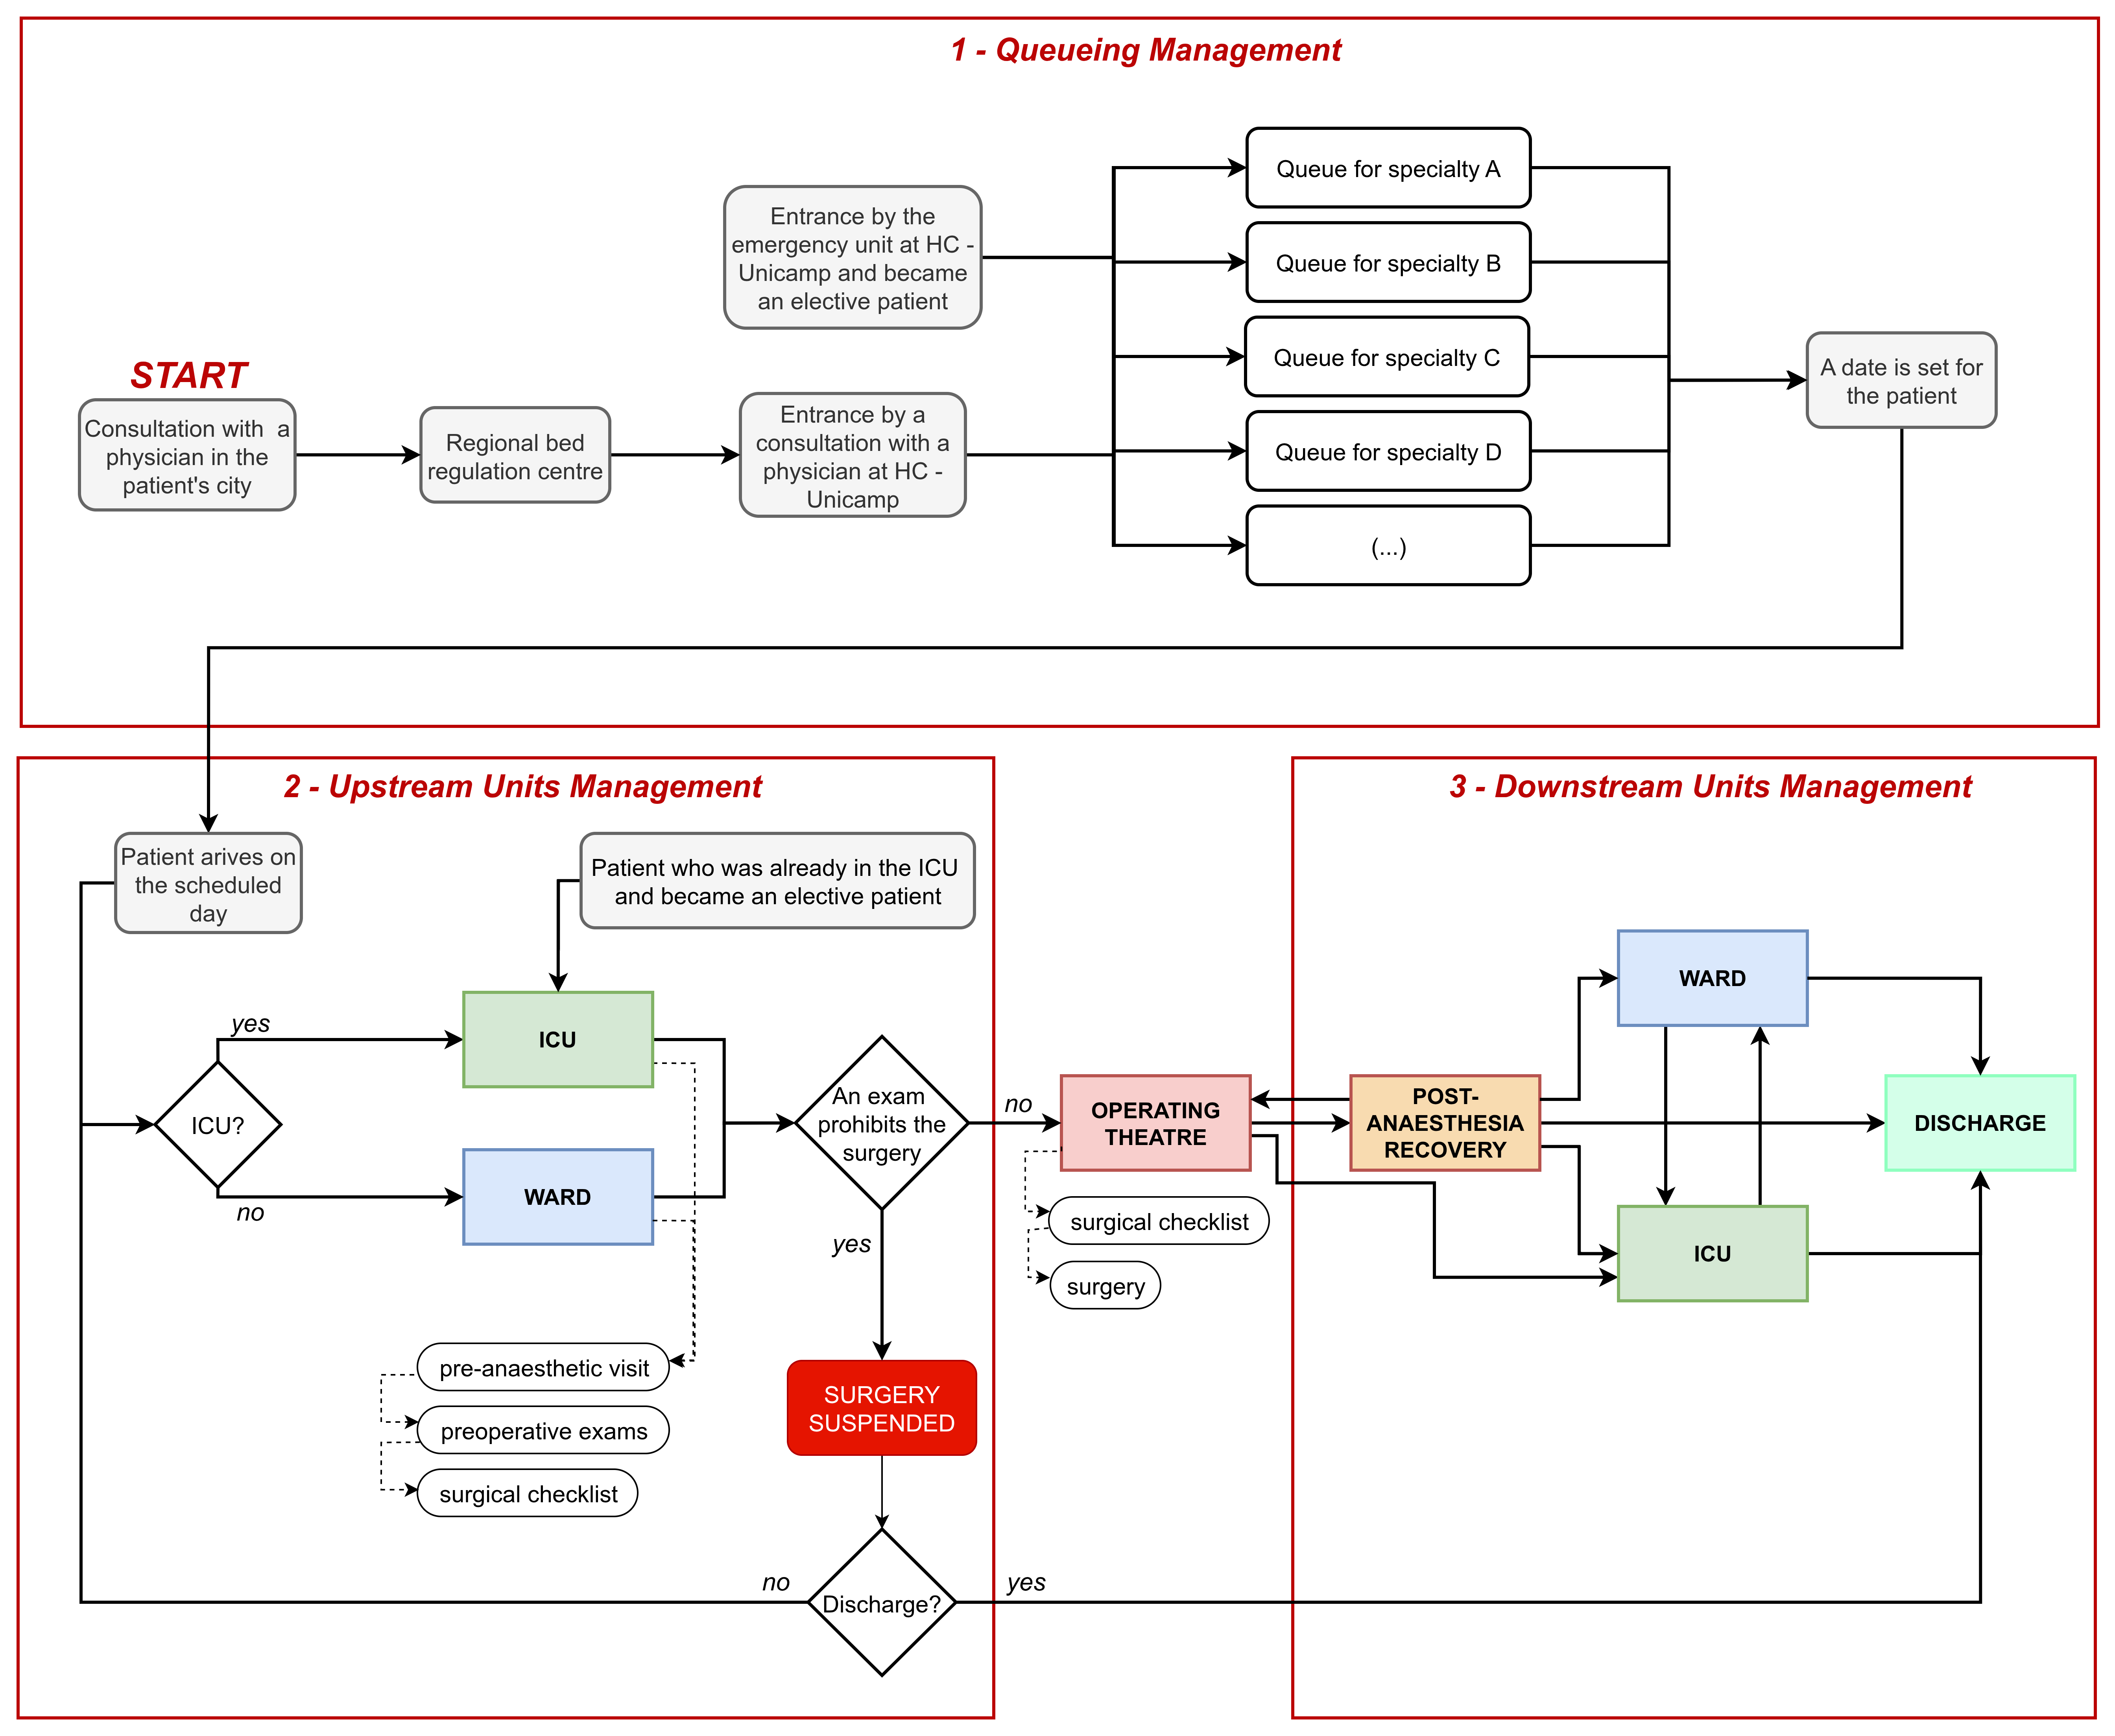
\includegraphics[width=0.9\textwidth]{images/patient_flow.png}
    \caption{Patient flow at HC - Unicamp.\label{fig:patient_flow}}
\end{figure}

On the day of surgery, patients enter the upstream unit management phase, where clinical reassessment is performed.
Depending on clinical requirements, Intensive Care Unit (ICU) support may be needed either pre- or post-operatively, requiring prior bed reservation; otherwise, ward bed availability must be ensured after surgery.
Patients then undergo pre-anaesthetic evaluation, diagnostic tests and surgical safety checks.
If contraindications arise, the procedure is suspended and the patient is either discharged or rescheduled, depending on clinical severity.
If cleared, the patient proceeds to the operating theatre, where the surgical procedure and subsequent theatre cleaning are performed.
In the present study, ward and ICU capacity are sufficient and therefore do not constitute binding constraints, allowing the analysis to focus on waiting-list management, surgery duration uncertainty and operating theatre allocation.

Once in the operating theatre, the patient is managed by a dedicated surgical team and anaesthetist.
This stage includes final safety checks, the surgical procedure itself and post-operative cleaning.
Here, uncertainty in surgery duration plays a central role, as it directly affects idle time, overtime and the risk of cancellations.
Consequently, surgery duration variability has a significant impact on operating theatre utilisation and overall system throughput, motivating its explicit consideration in the proposed framework.

Following surgery, patients are transferred to the Post-Anaesthesia Recovery Unit (PARU), with direct ICU transfer occurring only in exceptional cases.
After stabilisation, patients are admitted to a ward or ICU and subsequently discharged.
Although complications may occasionally require ICU readmission, recovery-unit capacity at HC-Unicamp is sufficient for the planning horizon considered.
This enables the proposed approach to concentrate on integrated waiting-list control, overtime management and operating theatre scheduling, in line with the contributions identified in the literature review.

HC-Unicamp operates $15$ operating theatres dedicated to elective surgeries: $13$ located in the Elective Surgery Centre (ESC) and $2$ in the Ambulatory Surgery Centre (ASC), which operates exclusively during morning shifts.
These theatres are heterogeneous with respect to infrastructure and equipment, leading to compatibility restrictions across medical subspecialties.

Each month, operating theatres must be allocated to $41$ medical subspecialties.
Relevant subsets include: (i) subspecialties requiring two consecutive time blocks; (ii) subspecialties with circumstantial but mandatory demand; (iii) priority subspecialties that take precedence in allocation decisions; and (iv) transplant subspecialties, which impose additional operational constraints.

The planning horizon comprises approximately $20$ working days per month, each divided into two shifts (morning and afternoon), defining $6$-hour time blocks.
Hospital policy assigns each block to a single subspecialty, while allowing the same subspecialty to occupy multiple blocks within the same theatre, provided compatibility conditions are met.
Sequential allocation is therefore permitted (and prefered by hospital managers), enabling a subspecialty assigned to a morning block to also occupy the corresponding afternoon block.

Allocation feasibility depends on the availability of surgical teams and anaesthetists.
A subspecialty can only be assigned to a block if an appropriate team is available on the corresponding day and shift.
Moreover, the number of simultaneous allocations requiring anaesthesia cannot exceed the number of anaesthetists available in each period.
For example, if $15$ anaesthetists are available on a given morning, at most $15$ anaesthesia-dependent procedures may be scheduled concurrently.

\begin{figure}[ht]
    \centering
    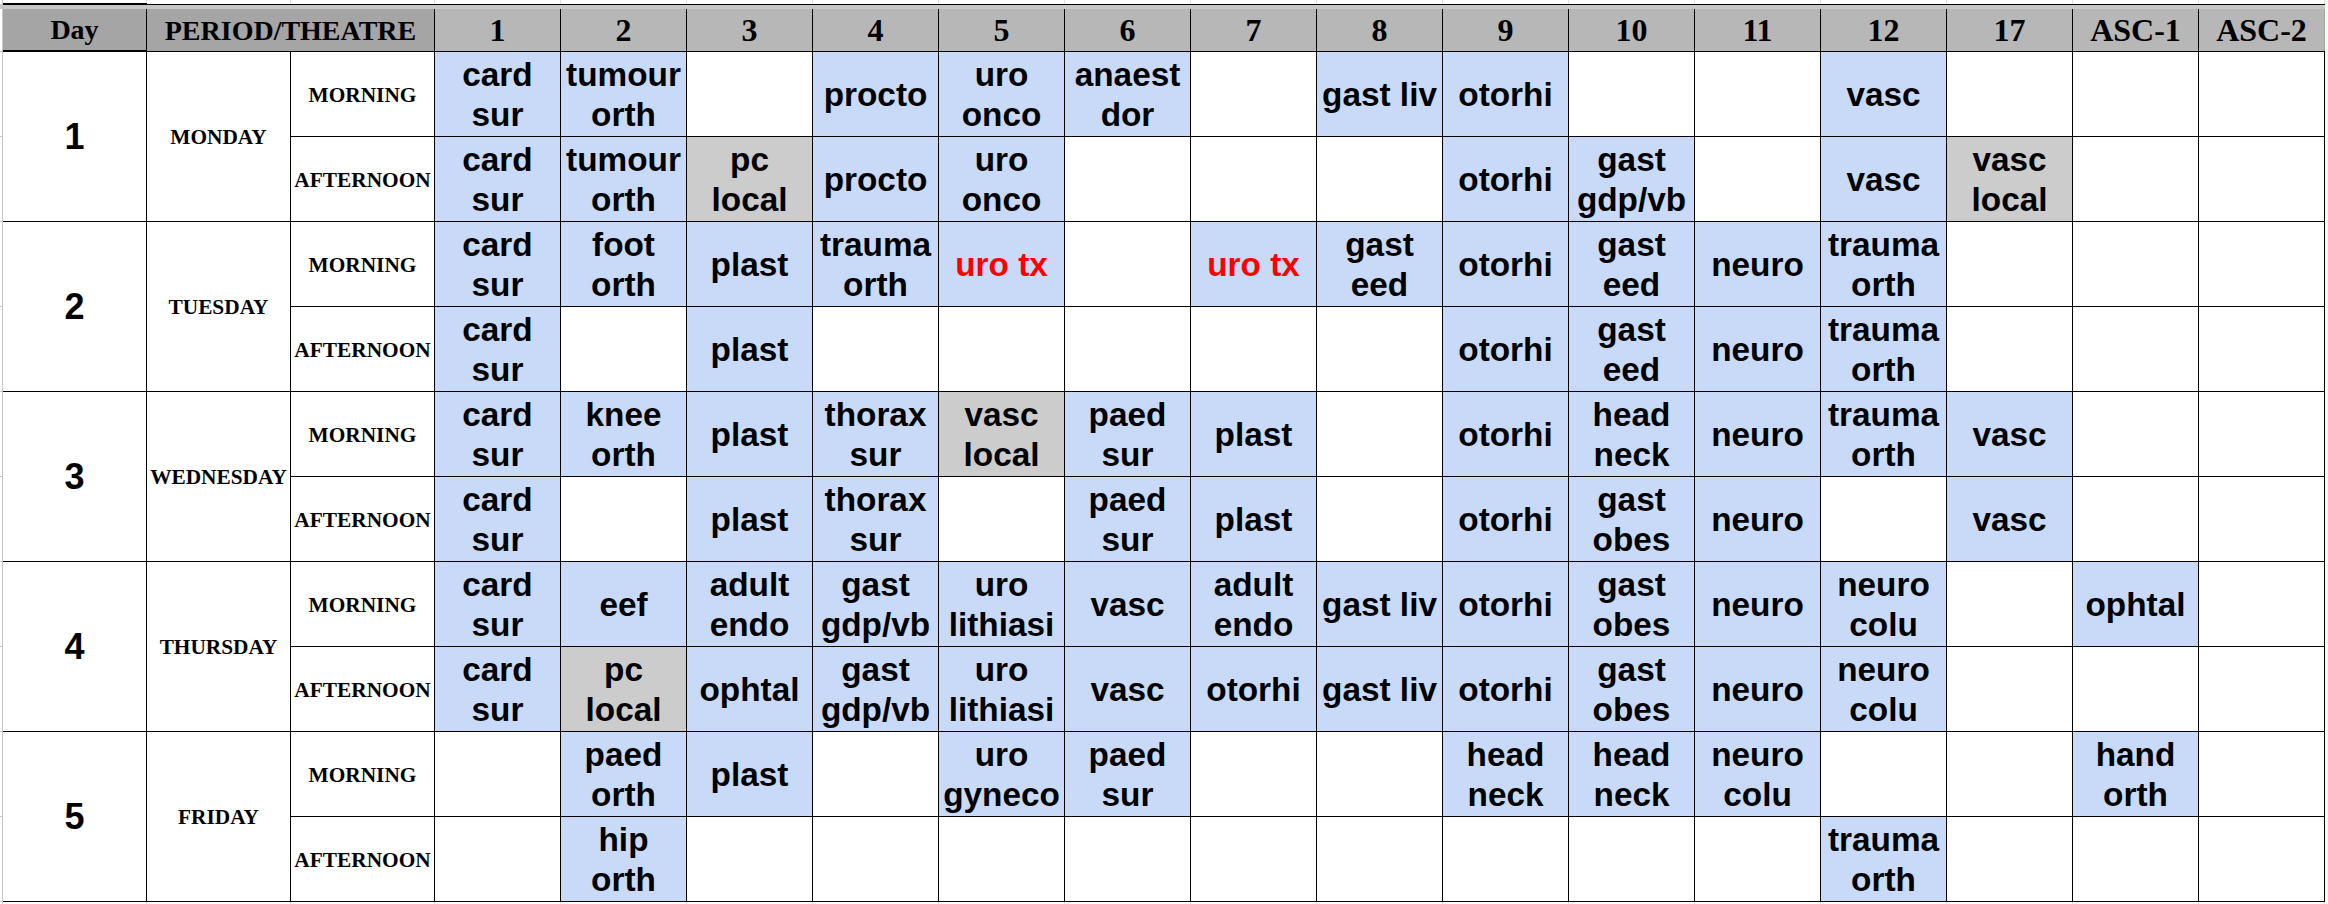
\includegraphics[width=0.9\textwidth]{images/trecho_escala.png}
    \caption{Excerpt from a week's operating theatre schedule.\label{fig:ex_escala}}
\end{figure}

Figure~\ref{fig:ex_escala} presents an excerpt from a weekly operating theatre schedule.
Rows represent time blocks and columns correspond to theatres; subspecialty allocations are colour-coded (blue for procedures requiring anaesthesia and grey otherwise).
Blank cells highlight unallocated slots, reflecting the complexity of the constraint set.
Allocations shown in red correspond to transplant surgeries, which require the simultaneous allocation of two theatres within the same time block.

Historically, schedules such as those shown in Figure~\ref{fig:ex_escala} have been manually constructed using spreadsheets, often requiring more than two full working day.
This manual process is time-consuming and does not guarantee optimality with respect to hospital policies and operational objectives.
Automating the scheduling process therefore reduces administrative burden and enables the generation of optimal or near-optimal solutions under complex constraints.

In this context, proposing an integrated planning framework for elective surgery at HC-Unicamp directly addresses the limitations identified in the literature.
By jointly managing waiting-list dynamics, surgery duration uncertainty and operating theatre allocation, the proposed approach provides a coherent and practically grounded solution capable of satisfying waiting-time requirements while mitigating idle time, overtime and cancellation risks.
%
% ********************************************
\section{Proposed Framework\label{sec:proposal}}
% *******************************************

We propose an integrated framework for elective surgery planning under uncertainty that links waiting-list management, in-block time management, and operating theatre scheduling. 
Rather than formulating these decisions as a single monolithic model, the framework decomposes the problem into three inter-related modules. 
The first two modules address strategic decisions related to queue and overtime management, and their outputs are then used as inputs to the tactical operating theatre scheduling model. 
Figure~\ref{fig:framework} summarises the proposed framework.

\begin{figure}[htb]
    \centering
    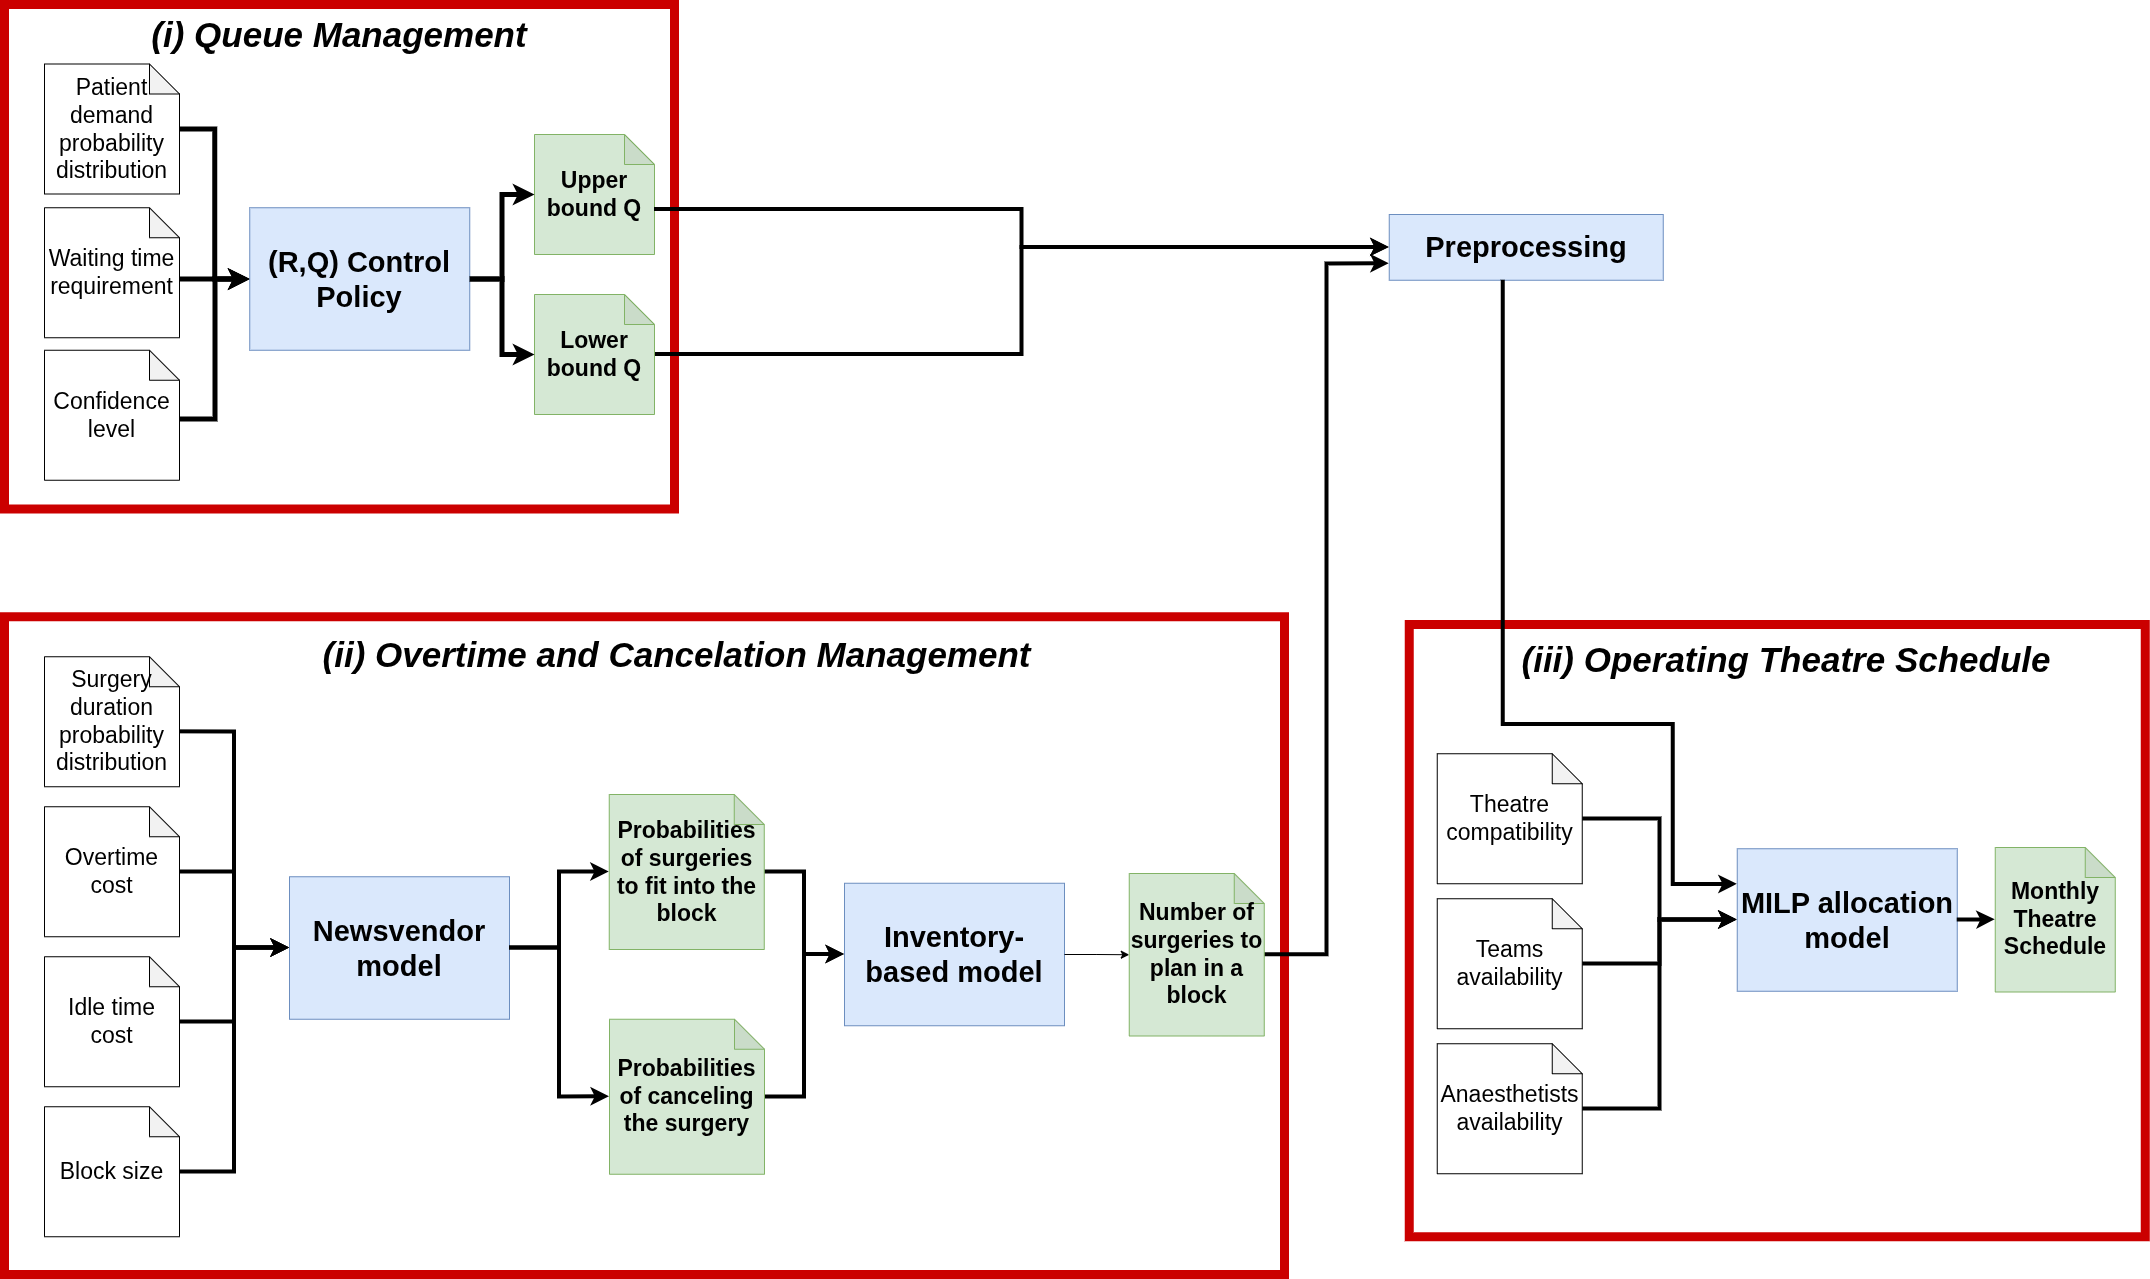
\includegraphics[width=0.9\textwidth]{images/framework.png}
    \caption{Proposed framework.\label{fig:framework}}
\end{figure}

The queue management module establishes targets for the number of surgeries to be performed at each planning period (e.g., monthly). 
Specifically, a modified $(R,Q)$ policy defines, for each medical sub-speciality, a lower and an upper bound on the number of patients to be admitted for surgery during the planning period, while ensuring that system-wide waiting-time requirements are satisfied in spite of the uncertainty in patient arrivals.
% This module supports the long-term balance of the waiting lists by aligning surgery admission with periodic patient arrivals via a classical inventory model under uncertainty.

The second module balances overtime, idle time and the risk of surgery cancellation due to overbooking. Considering the uncertainty in surgery duration, a Newsvendor model guides dynamic decisions on whether to perform or postpone the next surgery, given the time remaining in the session. The output of the Newsvendor model then informs an inventory model that determines the number of surgeries to be booked in a block while balancing the expected number of surgeries with the risk of cancellation.

The outputs of the first two modules are then combined to provide key inputs to the third module, which formulates the OT scheduling problem. 
Specifically, given the probability distribution of the number of performed surgeries per session (module 2), and the bounds on the number of surgeries to be performed in the period (module 1), one can derive lower and upper limits on the number of blocks to be allocated to each surgical sub-speciality. 
Hence, theatre allocation decisions are informed not only by resource availability and clinical compatibility, but also include constraints to guarantee that waiting-time requirements can be met despite the uncertainties in the demand and duration of surgeries. 
Crucially, the scheduling model remains deterministic, thereby facilitating practical implementation and ensuring rapid solution times.

Overall, the proposed framework provides a coherent approach to elective surgery planning across multiple decision levels.  By explicitly incorporating uncertainty into the strategic planning stages, it supports more robust and operationally meaningful scheduling decisions that are guaranteed to align to strategic waiting-time requirements. The following subsections present each module in detail. To help navigate the paper, Table~\ref{tab:acronyms} consolidates the list of acronyms. %For the mathematical notation, we refer the reader to the tables in each module's section.

\begin{table}[htb]
\centering
\caption{Acronyms used in the paper.\label{tab:acronyms}}
\scriptsize
    \begin{tabular}{ll}
        \toprule
        Acronym & Description \\
        \midrule
        CMP & Case Mix Planning \\
        MSS & Master Surgery Scheduling \\
        SCS & Surgical Case Scheduling \\
        OT  & Operating Theatre \\
        MDP & Markov Decision Process \\
        % SAA & Sample Average Approximation \\
        % DRO & Distributionally Robust Optimization \\
        SUS & Brazilian Unified Health System \\
        \hcunicamp & Hospital de Clínicas Unicamp \\
        OTSP & Operating Theatre Scheduling Problem \\
        MILP & Mixed-Integer Linear Programming \\
        PMF & Probability Mass Function \\
        CDF & Cumulative Distribution Function \\
        \bottomrule
    \end{tabular}
\end{table}
%
% ********************************************
\section{Long-Term Waiting List Management\label{sec:waitinglist}}
% *******************************************

As discussed in Section~\ref{sec:lit_review}, CMP constitutes the strategic decision layer responsible for determining the volumes of elective patients to be admitted over a given planning horizon.
In contrast to much of the existing literature, which primarily selects these volumes to optimise financial or capacity-related objectives, this work adopts a stability-oriented perspective.
We aim to enable decision-makers to impose maximum acceptable waiting times (e.g., six months) and to guarantee, in the long run, that such targets are met without allowing waiting lists to grow unboundedly. 
This is particularly relevant in the context of public healthcare systems, such as Brazil's Unified Health System (SUS), where there is a legal obligation to provide care to all patients in need.
Thus, ensuring equitable access to care and adherence to waiting time standards is paramount.

In line with this objective, this section introduces the theoretical foundations of the modified $(R,Q)$ control policy proposed to manage elective surgery waiting lists under stochastic demand.
We first characterise the dynamics of the underlying stochastic process and analyse its long-run behaviour. 
Subsequently, we derive analytical upper and lower bounds on the batch size $Q$ that ensures compliance with prescribed waiting-time requirements, thereby establishing the strategic input for the integrated planning framework.
Table~\ref{tab:symb_rq} summarises the notation used in this section.

\begin{table}[htb]
    \centering
    \caption{Symbols used in the long-term waiting list management model.\label{tab:symb_rq}}
    \scriptsize
    \begin{tabular}{cl}
    \toprule
    \textbf{Index} & \textbf{Description} \\
    \midrule
    $\stocprocperiod$ & Planning period index \\
    $\stocprocremainstate$ & State index of the remainder process \\
    $i,j$ & Generic state indices \\
    \midrule

    \textbf{Set} & \textbf{Description} \\
    \midrule
    $\statespace$ & State space of process $\stocprocqueue{\stocprocperiod}$ \\
    $\statespace_{\stocprocbatches{}}$ & State space of process $\stocprocbatches{\stocprocperiod}$ \\
    $\statespace_{\stocprocremain{}}$ & State space of process $\stocprocremain{\stocprocperiod}$ \\
    $\Omega$ & Support of the demand random variable \\
    \midrule

    \textbf{Parameter} & \textbf{Description} \\
    \midrule
    $\rthreshold$ & Reorder threshold of the modified $(R,Q)$ policy \\
    $\batchsizeq$ & Batch size under the modified $(R,Q)$ policy \\
    $\waittimereq$ & Waiting-time target \\
    $\conflevel$ & Probability threshold for the waiting-time requirement \\
    $\upq$ & Upper bound on feasible batch sizes \\
    $\lowq$ & Lower bound on feasible batch sizes \\
    $\maxnumberbatch$ & Maximum number of batch arrivals in one period \\
    \midrule

    \textbf{Random Variable / Stochastic Process} & \textbf{Description} \\
    \midrule
    $\stocprocqueue{\stocprocperiod}$ & Queue-length process \\
    $\rvdemand$ & Demand between two consecutive planning periods \\
    $\drawnrvdemand$ & Realisation of $\rvdemand$ \\
    $\stocprocbatches{\stocprocperiod}$ & Batch-level queue process \\
    $\stocprocremain{\stocprocperiod}$ & Remainder process associated with $\stocprocqueue{\stocprocperiod}$ \\
    $\roundbatches$ & Number of batch arrivals in one period \\
    $\omega$ & Waiting time of an arriving patient \\
    \midrule

    \textbf{Function} & \textbf{Description} \\
    \midrule
    $f_{\rvdemand}(\cdot)$ & Probability mass function of $\rvdemand$ \\
    $F_{\rvdemand}(\cdot)$ & Cumulative distribution function of $\rvdemand$ \\
    $\roundbatches(\stocprocremainstate)$ & Number of batch arrivals given remainder state $\stocprocremainstate$ \\
    $\steadystate{\stocprocremain{}}(\cdot)$ & Steady-state distribution of $\stocprocremain{\stocprocperiod}$ \\
    $\steadystate{\stocprocbatches{}}(\cdot)$ & Steady-state distribution of $\stocprocbatches{\stocprocperiod}$ \\
    $\transmatrix{\stocprocremain{}}$ & Transition matrix of process $\stocprocremain{\stocprocperiod}$ \\
    $\transmatrix{}^{\stocprocbatches{}}$ & Transition matrix of process $\stocprocbatches{\stocprocperiod}$ \\
    $\transmatrixval{\stocprocremainstate\stocprocremainstate'}{\stocprocremain{}}(k)$ & Conditional transition probability of $\stocprocremain{\stocprocperiod}$ given demand $k$ \\
    $\transmatrixval{ij}{}$ & Generic transition probability entry \\
    \midrule

    \textbf{Derived Quantity} & \textbf{Description} \\
    \midrule
    $\1_{\{\stocprocqueue{\stocprocperiod} \ge \rthreshold\}}$ & Indicator of batch processing \\
    \bottomrule
    \end{tabular}
\end{table}

% *******************************************
\subsection{$(R,Q)$ surgery scheduling policy: long-term distributions\label{sec:rqtheory}}
% *******************************************

Let $\stocprocqueue{\stocprocperiod}, \, \stocprocperiod \ge 0$ be a stochastic process representing an elective surgery queue with stationary and independent increments over discrete planning periods, with $\stocprocqueue{\stocprocperiod}$ representing the number of patients in the system at period $\stocprocperiod \ge 0$. Assume that the queue is controlled via a modified $(R,Q)$ policy \citep[e.g.,][]{Axsater2015Inv} whereby a batch of $\batchsizeq \in \mathbb N$ surgeries is processed at time period $\stocprocperiod$ whenever $\stocprocqueue{\stocprocperiod} \ge \rthreshold, \, \rthreshold \ge \batchsizeq$ at the start of the period, where $\mathbb N$ is the set of positive integers. In contrast to the classical $(R,Q)$ policy, which processes as many batches as necessary to bring the inventory below the reorder point ($R$), our policy can only process a batch at a time and relies on long-term properties to ensure that the process $\stocprocqueue{\stocprocperiod}, \, \stocprocperiod \ge 0$ is stable and guarantees prescribed waiting time requirements.

Let $\rvdemand$ be a non-negative integer random variable representing the overall demand between two consecutive planning periods, with probability distribution $f_{\rvdemand}: \Omega \to [0,1), \, \Omega \subset \mathbb Z_+$, and cumulative distribution $F_{\rvdemand}: \mathbb Z_+ \to [0,1]$ given by
%
\[
F_{\rvdemand}(d) = \sum_{l=0}^{\drawnrvdemand} f_{\rvdemand}(l),
\]
%
where $\mathbb Z_+$ denotes the set of non-negative integers. This implies that the dynamics of process $\stocprocqueue{\stocprocperiod}, \, \stocprocperiod \ge 0$ can be expressed as:
%
\begin{equation} \label{eq:dynamics}
\stocprocqueue{\stocprocperiod+1} = \stocprocqueue{\stocprocperiod} + \drawnrvdemand - \batchsizeq \1_{\{\stocprocqueue{\stocprocperiod} \ge \rthreshold\}},
\end{equation}
%
where $\1_{\{A\}}$ is the indicator function, which is equal to $1$ if $A$ holds and is nil otherwise, and $\drawnrvdemand$ is a value drawn from $f_{\rvdemand}$ that represents the surgical demand in period $\stocprocperiod$. The state space of process $\stocprocqueue{\stocprocperiod}, \, \stocprocperiod \ge 0$ is given by $\statespace = \{ 0, \, 1 , \, 2, \, \ldots \}$, where $\stocprocqueue{\stocprocperiod}=i$ indicates that there are $\rthreshold-\batchsizeq + i$ patients waiting for elective surgery.

Letting 
%
\begin{equation} \label{eq:defYZ}
\stocprocbatches{\stocprocperiod} = \left \lfloor \dfrac{\stocprocqueue{t}}{Q} \right \rfloor, \qquad Z_t = \stocprocqueue{t} \, \% \,  \batchsizeq,
\end{equation}
%
where $\%$ represents the modulus operator, we can write:
%
\[
\stocprocqueue{\stocprocperiod} = Q \stocprocbatches{\stocprocperiod} + \stocprocremain{\stocprocperiod},
\]
% 
where $\stocprocbatches{\stocprocperiod}, \, \stocprocperiod \ge 0$ is the integer number of batches required to bring the queue instantaneously below $\rthreshold$ and $\stocprocremain{\stocprocperiod} \in \{0, 1, \ldots, \batchsizeq-1\}$ is the number of patients that would remain in excess of the minimum allowed queue of $(\rthreshold-\batchsizeq)$ patients after removing $\stocprocbatches{\stocprocperiod}$ batches of $\batchsizeq$ patients instantaneously.

Note that, from the definitions above, the state space of process $\stocprocbatches{\stocprocperiod}, \, \stocprocperiod \ge 0$ is $\statespace_{\stocprocbatches{}} = \mathbb Z_+$, while $\statespace_{\stocprocremain{}} = \{0, \, 1, \, \ldots, \, Q-1\}$ is the state space of process $\stocprocremain{\stocprocperiod}, \, \stocprocperiod \ge 0$. In the next result, we will derive the long-term distribution of process $\stocprocremain{\stocprocperiod}, \, \stocprocperiod \ge 0$.

\begin{prop} \label{prop:steadystate}
Let $\steadystate{\stocprocremain{}}: \statespace_{\stocprocremain{}} \to [0,1]$ be the steady state distribution of process $\stocprocqueue{\stocprocperiod}, \, \stocprocperiod \ge 0$. Then, it holds that 
%
\begin{equation} \label{eq:steadyZ}
\steadystate{\stocprocremain{}}(\stocprocremainstate) = \dfrac{1}{\batchsizeq}, \forall \stocprocremainstate \in \statespace_{\stocprocremain{}}.
\end{equation}
%
\end{prop}
%
\begin{proof}
The proof closely follows that of \citet[Proposition 5.1]{Axsater2015Inv}. Let $\transmatrix{\stocprocremain{}}$ be the transition matrix describing the dynamics of process $\stocprocremain{\stocprocperiod}, \, \stocprocperiod \ge 0$. Assume that $\stocprocremain{\stocprocperiod} = \stocprocremainstate, \, \stocprocremainstate \in \statespace_{\stocprocremain{}}$ at the start of period $\stocprocperiod \ge 0$, and let and $\rvdemand=k$ be the number of new patient arrivals in period $\stocprocperiod$. Hence, it follows that 
%
\[
\stocprocremain{\stocprocperiod+1} =  (\stocprocremainstate + k) \,\%\, \batchsizeq  = (\stocprocremainstate + k + \batchsizeq \stocprocbatches{\stocprocperiod}) \,\%\, \batchsizeq  = (\stocprocqueue{\stocprocperiod} + k) \,\%\, \batchsizeq,
\] 
%
where the last equality come from the definitions in Eq.~\eqref{eq:defYZ}. Therefore, given $\rvdemand=k$, it is evident that $\transmatrixval{\stocprocremainstate\stocprocremainstate'}{\stocprocremain{}}(k) := P( \stocprocremain{\stocprocperiod+1} = \stocprocremainstate' | \stocprocremain{\stocprocperiod} = \stocprocremainstate, \rvdemand=k )$ equals one for exactly one value of $\stocprocremainstate$ and zero otherwise. Consequently, we can write:
%
\[
\sum_{\stocprocremainstate=0}^{\batchsizeq-1} \transmatrixval{\stocprocremainstate\stocprocremainstate'}{\stocprocremain{}} = \sum_{\stocprocremainstate=0}^{\batchsizeq-1} \mathbb{E}_{k} \left\{ \transmatrixval{\stocprocremainstate\stocprocremainstate'}{\stocprocremain{}}(k) \right\} = \mathbb{E}_k \left\{  \sum_{\stocprocremainstate=0}^{\batchsizeq-1} \transmatrixval{\stocprocremainstate\stocprocremainstate'}{\stocprocremain{}}(k) \right\} = \mathbb{E}_k \{ 1 \} = 1.
\]
%
The expression above  implies that the Markov chain describing the dynamics of process $Z_t, \, t \ge 0$ is doubly stochastic, and therefore has a uniform steady state distribution. Indeed, substituting \eqref{eq:steadyZ} in the steady state equations:
%
\[
\steadystate{}^{\stocprocremain{}}(\stocprocremainstate) = \sum_{\stocprocremainstate'=0}^{\batchsizeq-1} \steadystate{}^{\stocprocremain{}}(\stocprocremainstate') \transmatrixval{\stocprocremainstate'\stocprocremainstate}{\stocprocremain{}},
\]
%
one can easily see that the steady state distribution satisfies Eq. \eqref{eq:steadyZ}.
%
\end{proof}

The result in Proposition \ref{prop:steadystate} is very important, as it shows that the steady state distribution of process $\stocprocremain{\stocprocperiod}, \, \stocprocperiod \ge 0$, is uniform regardless of the distribution of patient arrivals. Next, we will use this fact to derive the steady state distribution of process $\stocprocbatches{\stocprocperiod}, \, \stocprocperiod \ge 0$. 

% ********************************************
\subsection{The dynamics of process $\stocprocbatches{\stocprocperiod}, \, \stocprocperiod \ge 0$\label{sec:batchprocess}}
% *******************************************

Assume that process $\stocprocremain{\stocprocperiod}, \, \stocprocperiod \ge 0$ has reached equilibrium, which is also equivalent to supposing that $P(\stocprocremain{0} = \stocprocremainstate) = \steadystate{\stocprocremain{}}(\stocprocremainstate) = \dfrac{1}{\batchsizeq}$ \citep[e.g.,][]{Bremaud2020}. We can describe the dynamics of process $\stocprocbatches{\stocprocperiod}, \, \stocprocperiod \ge 0$ as:
%
\begin{equation} \label{eq:dynY}
\stocprocbatches{\stocprocperiod+1} = \begin{cases}
\stocprocbatches{\stocprocperiod} - 1 + \roundbatches, & \text{if} \; \stocprocbatches{\stocprocperiod} \ge 0, \\
\roundbatches; \; & \text{if} \; \stocprocbatches{\stocprocperiod} = 0,
\end{cases}
\end{equation}
%
where $\roundbatches$ is the round number of batch arrivals at time $\stocprocperiod$. To fully characterize the random variable $\roundbatches$, it is necessary to define
%
\begin{equation} \label{eq:Az}
\roundbatches(\stocprocremainstate) = \left \lfloor \dfrac{\rvdemand + \stocprocremainstate}{\batchsizeq} \right \rfloor,
\end{equation}
%
which represents the round number of batch arrivals at time $\stocprocperiod$, given that $\stocprocremain{\stocprocperiod} = \stocprocremainstate$. Then, in view of Proposition~\ref{prop:steadystate}, it follows that:
%
\begin{equation} \label{eq:batcharr}
P(\roundbatches = k ) = \dfrac{1}{\batchsizeq} \sum_{\stocprocremainstate=0}^{\batchsizeq-1} P(\roundbatches(\stocprocremainstate) = k ).    
\end{equation}

Therefore, from \eqref{eq:dynY} we have:
%
\begin{equation} \label{eq:ydynamicY}
\transmatrixval{ij}{\stocprocbatches{}} = P(\stocprocbatches{\stocprocperiod+1} = j | \stocprocbatches{\stocprocperiod} = i ) = \begin{cases}
    P\left( \roundbatches = j  \right), & \text{if} \; \stocprocbatches{\stocprocperiod} = 0, \\
    P\left( \roundbatches = j-i + 1 \right),  & \text{if} \; \stocprocbatches{\stocprocperiod} \ge 1.
\end{cases}
\end{equation}
%

Note that Eq. \eqref{eq:dynY}-\eqref{eq:ydynamicY} correspond to the dynamics in \citet[Section 6.1.2]{Shortle2018}. Similarly to \citet{Shortle2018}, the transition matrix of process $\stocprocbatches{\stocprocperiod}, \, \stocprocperiod \ge 0$ can be written as:
%
\begin{equation}
\transmatrix{}^{\stocprocbatches{}} = [\transmatrixval{ij}{}] = \left[
\begin{array}{cccccccc}
k_0 & k_1 & k_2 & \ldots & k_M & 0 & 0 & \ldots \\
k_0 & k_1 & k_2 & \ldots & k_M & 0 & 0 & \ldots \\
0 & k_0 & k_1 & k_2 & \ldots & k_M & 0 & \ldots \\
0 & 0 & k_0 & k_1 & k_2 & \ldots & k_M & \ldots \\
\vdots & \vdots & \vdots & \vdots & \vdots & \vdots & \vdots & 
\end{array}
\right],
\end{equation}
%
where $\maxnumberbatch$ is the maximum number of new batch arrivals, i.e., the maximum value that random variable $\roundbatches$ can assume.

The steady state probabilities of process $\stocprocbatches{\stocprocperiod}, \, \stocprocperiod \ge 0$ can then be recursively evaluated by solving:
\begin{equation} \label{eq:ssY}
\steadystate{\stocprocbatches{}}^T = \steadystate{\stocprocbatches{}}^T P,
\end{equation}
%
with the contour condition that $\steadystate{\stocprocbatches{}}(0) = 1 - \rho $ \citep[Eq. (6.12)]{Shortle2018}, 
%
%\begin{equation} \label{eq:ssY}
%\pi_Y(i) = \begin{cases}
%1 - \rho, & \text{if} \; i = 0, \\
%(1 - \rho) k_i + \displaystyle \sum_{j=1}^{i+1} \pi_Y(j) k_{i-j+1}, \, i \ge 0
%\end{cases}
%\end{equation}
%
where $\rho = E(\roundbatches)$. Observe that, to guarantee stability, we must have $E(\roundbatches) < 1$. Note also that the steady state probabilities up to a given state $j$ can be recursively calculated using the first $j$ equations in \eqref{eq:ssY}.

% ********************************************
\subsection{Upper and lower bounds on the batch size $\batchsizeq$ under waiting time requirements} \label{sec:bounds}
% *******************************************

Let $\omega$ be the waiting time of a patient joining the queue, and assume that the healthcare system requires that:
%
\begin{equation} \label{eq:waitthreshold}
P( \omega > \tau ) < \alpha,
\end{equation}
%
for some target waiting time $\waittimereq >0$ and probability threshold $\conflevel \in (0,1)$. Now, if a patient arrives and encounters $\stocprocbatches{\stocprocperiod} > 0$ batches of patients in the queue, their turn will only arrive once these $\stocprocbatches{\stocprocperiod}$ batches are processed, which will take $\stocprocbatches{\stocprocperiod}$ time periods. This means that the patient will have to wait $\waittimereq = \stocprocbatches{\stocprocperiod}$ periods for their turn. Therefore, Eq. \eqref{eq:waitthreshold} can be equivalently stated as:
%
\begin{equation} \label{eq:waitthresholdy}
\sum_{i = 0}^\waittimereq \steadystate{\stocprocbatches{}}(i) > 1 - \conflevel,
\end{equation}
%
where $\steadystate{\stocprocbatches{}} : \statespace_{\stocprocbatches{}} \to (0,1)$ satisfies Eq. \eqref{eq:ssY}. Therefore, to limit the waiting time according to the prescribed requirements, we can establish a lower bound ($\lowq$) on the batch size $\batchsizeq > 0$ as follows:
%
\begin{equation} \label{eq:under}
\lowq = \min \{ \batchsizeq \in \mathbb N : \sum_{i = 0}^\waittimereq \steadystate{\stocprocbatches{}}(i) > 1- \conflevel \}.
\end{equation}

When $\stocprocbatches{\stocprocperiod} = 0$, on the other hand, the next batch will only be processed when the system leaves this state, therefore by applying the strong Markov property \citep{Bremaud2020}, we have:
%
\[
\omega = \min \{\delta > 0 : \stocprocbatches{\delta} > 0 | \stocprocbatches{0} = 0 \}.
\]
%
Considering the transition matrix in Eq.~\eqref{eq:ydynamicY}, it follows that $\omega$ will be a geometrically distributed variable and:
%
\begin{equation} \label{eq:upperbound}
P( \omega > \waittimereq | \stocprocbatches{0} = 0 )  = k_0^{\waittimereq}.
\end{equation}

One can intuitively see that the value of $k_0$ will increase as $\batchsizeq$ increases, since in this case we will need more patient arrivals until we are able to process a full batch of patients. Hence, from Eq. \eqref{eq:upperbound}, we can set up an upper bound $\upq$ for the batch size such that:
%
\begin{equation} \label{eq:overbound}
\upq = \max \{ \batchsizeq \in \mathbb N : k_0^{\waittimereq} < \conflevel \}.
\end{equation}


% Therefore, considering a set of medical subspecialties $\specialtyset$, we can calculate batch sizes $\upq_{\specialtyidx}$ and $\lowq_{\specialtyidx}$ for every specialty $\specialtyidx \in \specialtyset$, and then ensure that the waiting time requirements are satisfied both when patients arrive to an empty queue and when they encounter batches of patients in the queue.
In the example below, we show how to derive general bounds $\lowq$ and $\upq$ for a given demand distribution and waiting time requirements.

\begin{ex}[Deriving lower and upper bounds for $\batchsizeq$]
Consider an elective surgery queue with monthly demand $\rvdemand$ that satisfies the distribution in Table \ref{tab:demprob}.
%
\begin{center}
\begin{table}[h!]
\caption{Monthly demand distribution for surgeries} \label{tab:demprob}
\scriptsize{
\begin{tabular}{|l|c|c|c|c|c|c|c|c|c|c|c|} \hline \hline
\textbf{Demand ($\drawnrvdemand$)} & 0 & 1 & 2 & 3 & 4 & 5 & 6 & 7 & 8 & 9 & 10 \\ \hline
$P(\rvdemand=\drawnrvdemand)$ & 0.0308 & 0.0393 & 0.1179 & 0.2096 & 0.2445 & 0.1956 & 0.1086 & 0.0414 & 0.0103 & 0.0015 & 0.0005 \\ \hline
\end{tabular}
}
\end{table}
\end{center}
%
The expected monthly demand is therefore $\mathbb{E}(\rvdemand) = 3.9022$. Setting $\batchsizeq = 4$, which ensures long-term stability, we have $\statespace_{\stocprocremain{}{}} = \{0, 1, 2, 3\}$. This allows us to evaluate the individual distributions of $\roundbatches(\stocprocremainstate), \, \stocprocremainstate \in \statespace_{\stocprocremain{}}$ as defined in Eq. \eqref{eq:Az}, which we depict in the Table \ref{tab:dembatches}, along with the distribution of variable $\roundbatches$ from Eq. \eqref{eq:batcharr}.


\begin{table}[h!]
\centering \caption{Monthly demand distribution for surgeries} \label{tab:dembatches}
\scriptsize{
\begin{tabular}{|l|c|c|c|c|} \hline \hline
$P(\roundbatches(\stocprocremainstate) = \drawnrvdemand) $ & \multicolumn{4}{|c|}{\textbf{Batch demand ($\drawnrvdemand$)}} \\ \cline{2-5}
  & 0 & 1 & 2 & 3 \\ \hline
$\stocprocremainstate=0$   & 0.3976 & 0.5901 & 0.0123 & 0 \\ \hline
$\stocprocremainstate=1$   & 0.1880 & 0.7583 & 0.0537 & 0 \\ \hline
$\stocprocremainstate=2$   & 0.0701 & 0.7676 & 0.1618 & 0.0005 \\ \hline
$\stocprocremainstate=3$   & 0.0308 & 0.6113 & 0.3559 & 0.002 \\ \hline
\textbf{$P(\roundbatches=\drawnrvdemand)$} & \textbf{0.171625} &  \textbf{0.681825} & \textbf{0.145925} &  \textbf{0.000625} \\ \hline
\end{tabular}
}
\end{table}

The distributions in Table \ref{tab:dembatches} follow directly from Eq. \eqref{eq:Az} and Eq. \eqref{eq:batcharr}. For example, when $\stocprocremainstate=0$, we know that the queue comprises an integer number of batches. Therefore, $P(\roundbatches(0) = 0) = p_{\rvdemand}(0) + p_{\rvdemand}(1) + p_{\rvdemand}(2) + p_{\rvdemand}(3)$ (Table \ref{tab:demprob}) as up to 3 new arrivals will not suffice to generate a new batch of $Q=4$ patients. Analogously, $\roundbatches(0)=1$ if we observe from 5 to 7 arrivals and $\roundbatches(0)=2$ when 8 to 10 patients arrive in the period, as these will suffice for 2 new batches. 

Conversely, when $\stocprocremainstate=3$, we have three patients in excess of a discrete number of batches, which means that $P(\roundbatches(3) = 0) = p_{\rvdemand}(0)$ as new batches will be formed whenever one or more patients arrive. One new batch will form if $\rvdemand \in [1,4]$, two new batches if $\rvdemand \in [5,8]$ and three new batches when $\rvdemand \in [8,10]$. Specifically, when 10 patients arrive, they will form a set of 13 patients when joined to the $\stocprocremainstate=3$ remaining patients from the start of the period. These 3 patients will then suffice to form three batches of $\batchsizeq=4$ patients, with one remaining batchless for the following period.

Note that $\mathbb{E}(\roundbatches) = 0.9755$, and that this value is equal to $\rho = \dfrac{\mathbb{E}(\rvdemand)}{\batchsizeq} = \dfrac{3.9022}{4} = 0.9755$. This is expected, as the dynamics of process $\stocprocbatches{\stocprocperiod}$ describes the original system, only looking at it in terms of batches of patients. Note that $\mathbb{E}(\roundbatches)$ is simply the expected number of batches of $\batchsizeq$ patients arriving and since we process $\mu=1$ batch per time period, we have $\rho = \mathbb{E}(\roundbatches)$ when looking at the evolution of the batch process $\stocprocbatches{\stocprocperiod}, \, \stocprocperiod \ge 0$.

Now, let us suppose that $\waittimereq = 6$ and $\conflevel = 0.05$ in~\eqref{eq:waitthreshold}, which means that the system requires 95\% of the patients to be operated in up to six months. To verify whether that is satisfied, we need firstly to solve Eq. \eqref{eq:ssY} for the steady state distribution of $\stocprocbatches{\stocprocperiod}, \, \stocprocperiod \ge 0$ and then use it to verify~\eqref{eq:waitthresholdy}. From Table~\ref{tab:dembatches}, we obtain $k_0=0.171625$,  $k_1=0.681825$, $k_2 = 0.145925$ and $k_3=0.000625$, which can be applied in Eq.~\eqref{eq:ssY} to find $\steadystate{\stocprocbatches{}}(0) = 0.02445$, $\steadystate{\stocprocbatches{}}(1) = 0.1182$, $\steadystate{\stocprocbatches{}}(2) = 0.1219$, $\steadystate{\stocprocbatches{}}(3) = 0.1046$, $\steadystate{\stocprocbatches{}}(4) = 0.0898$, $\steadystate{\stocprocbatches{}}(5) = 0.077$, $\steadystate{\stocprocbatches{}}(6) = 0.0661$. This yields:
\[
P(\omega \le 6 | \stocprocbatches{\stocprocperiod} \ge 1) \approx 0.602 < 0.95 = 1 - \alpha.
\]
%
This implies that $\underline Q > 4$ in Eq. \eqref{eq:under} and we should, therefore, recalculate the probability above for increasing values of $Q$ until we find the first value that satisfies the waiting time criterion - which will give us the lower bound $\underline Q$.

To verify the waiting time requirements when $\stocprocbatches{\stocprocperiod} = 0$, one can apply \eqref{eq:upperbound}, which implies that $P(\omega \le 6 | \stocprocbatches{\stocprocperiod} = 0) = 0.171625^6 \approx 2.5 \cdot 10^{-5} < 0.05$. Therefore, to find the bound $\overline Q$ in Eq. \eqref{eq:overbound}.

When verifying Eq.~\eqref{eq:under} with $Q = 10$, it implies $P(\omega \le 6 | \stocprocbatches{\stocprocperiod} = 0) = 0.609780^6 \approx 0.05114 > 0.05$. Then, if one set $\batchsizeq = 9$, it implies $P(\omega \le 6 | \stocprocbatches{\stocprocperiod} = 0) = 0.566478^6 \approx 0.03304 < 0.05$. Thus, we can set $\upq = 9$.

For the $\lowq$, one can verify $\batchsizeq = 5$, which implies $k_0=0.265720$,  $k_1=0.688120$, $k_2 = 0.046160$ and $k_3=0$, which can be applied in Eq. \eqref{eq:ssY} to find $\steadystate{\stocprocbatches{}}(0) = 0.21956$, $\steadystate{\stocprocbatches{}}(1) = 0.606723$, $\steadystate{\stocprocbatches{}}(2) = 0.143539$, $\steadystate{\stocprocbatches{}}(3) = 0.024935$, $\steadystate{\stocprocbatches{}}(4) = 0.004332$, $\steadystate{\stocprocbatches{}}(5) = 0.000752$, $\steadystate{\stocprocbatches{}}(6) = 0.000131$. This yields:
\[
P(\omega \le 6 | \stocprocbatches{\stocprocperiod} \ge 1) \approx 0.999973 > 0.95 = 1 - \alpha.
\]
%
Thus, we can set $\lowq = 5$.
%
%
\end{ex}
%
% ********************************************
\section{Estimating the number of patients per time block}
% *******************************************

To ensure consistency with the waiting-time requirements established by the $(R,Q)$ policy in Section~\ref{sec:waitinglist}, it is necessary to estimate how many elective patients can be accommodated within a single $6$-hour operating theatre block, in accordance with the scheduling regulations at HC-Unicamp. 
This estimation determines whether the batch sizes $\upq$ and $\lowq$, for each specialty $\specialtyidx \in \specialtyset$, defined at the strategic level can be effectively served within the planning horizon.

Accurate estimation requires explicit consideration of uncertainty in surgery durations, which varies across subspecialties and directly affects both operating theatre utilisation and the risk of overtime. 
In particular, a trade-off arises between idle time, resulting from underutilised theatre capacity, and overtime, which may trigger cancellations of scheduled procedures. 

For this purpose, in this section we present the second module of the proposed integrated framework. 
A newsvendor-based model is first employed to determine an optimal time allocation for the final surgery in a block under duration uncertainty, balancing idle-time and overtime costs. 
Building on this result, an inventory-based formulation is then used to estimate the number of patients that can be reliably scheduled within a time block, providing the tactical input required for subsequent operating theatre allocation decisions.
The symbols used in this section are defined in Table~\ref{tab:symb_newsvendor}.

\begin{table}
    \centering
    \caption{Table of Symbols for Overtime and cancellation management process.\label{tab:symb_newsvendor}}
    \scriptsize
    \begin{tabular}{cl}
    \toprule
    % \textbf{Index} & \textbf{Description} \\
    % \midrule
    % $\surgidx$ & Surgery index \\
    % $\completedsurgsidx$ & Number of completed surgeries \\
    % $\cancellationsidx$ & Number of cancellations \\
    % \midrule
    \textbf{Parameter} & \textbf{Description} \\
    \midrule
    $\blocklength$ & Length of the surgery block (hours) \\
    $\safetythreshold$ & Safety time threshold required to start a new surgery, resulting from the Newsvendor model \\
    $\probstoppingthreshold$ & Probability threshold used as stopping criterion in the algorithm \\
    $\plannedsurgs$ & Number of surgeries planned for a block of length $\blocklength$, such that $\plannedsurgs \in \mathbb{N}_+$ \\
    $\durationpmf$ & Discretised probability mass function of a single surgery duration \\
    \midrule
    \textbf{Random Variable} & \textbf{Description} \\
    \midrule
    $\duration_{\surgidx}$ & Duration of the ${\surgidx}$-th surgery \\
    $\cumulativeduration{\completedsurgsidx}$ & Cumulative duration of the first $\completedsurgsidx$ surgeries, $\cumulativeduration{\completedsurgsidx} = \sum_{i=1}^{\completedsurgsidx} \duration_i$ \\
    $\numcompletedsurgs$ & Number of surgeries performed within the block \\
    \midrule
    \textbf{Function} & \textbf{Description} \\
    \midrule
    $F_{\cumulativeduration{\completedsurgsidx}}(\cdot)$ & Cumulative distribution function of $\cumulativeduration{\completedsurgsidx}$ \\
    $\convolve(\cdot,\cdot)$ & Convolution operator used to compute cumulative duration distributions \\
    $\runnewsvendor(\cdot)$ & Function to compute $P(\cumulativeduration{\completedsurgsidx} < \blocklength - \safetythreshold)$\\
    $\gain(\cdot)$ & Gain function associated with scheduling additional surgeries \\
    $\cancellationcost(\cdot)$ & Cost function associated with cancellations \\
    $\netvalue(\cdot)$ & Net value function combining gain and cancellation cost \\
    $\marginalvalue(\cdot)$ & Marginal value function for scheduling additional surgeries \\
    $\cancellationfunction(\cdot)$ & Function to compute cancellation probabilities \\
    \midrule
    \textbf{Derived Quantity} & \textbf{Description} \\
    \midrule
    $P(\plannedsurgs > \completedsurgsidx)$ & Probability that more than $\completedsurgsidx$ surgeries can be completed (survival function)\\
    $P(\plannedsurgs = \completedsurgsidx)$ & Probability that exactly $\completedsurgsidx$ surgeries can be completed \\
    $K_{\max}$ & Maximum number of surgeries considered, such that $F_{\cumulativeduration{\completedsurgsidx}}(\blocklength - \safetythreshold) > \probstoppingthreshold$ \\
    $q[k]$ & Discrete representation of $P(\numcompletedsurgs > \completedsurgsidx)$ (survival function of $\numcompletedsurgs$) \\
    $c^{(k)}$ & Probability distribution of cumulative duration $\cumulativeduration{\completedsurgsidx}$ \\
    \midrule
    \textbf{Output Metric} & \textbf{Description} \\
    \midrule
    $P(\text{cancellations} = \cancelledsurgeries)$ & Probability that $\cancelledsurgeries$ surgeries are cancelled \\
    \bottomrule
    \end{tabular}
\end{table}

% ********************************************************************************************* %
\subsection{Managing surgery cancellations via a newsvendor-based model\label{sec:cancel}}
% ********************************************************************************************* %

Let us now consider the problem of determining the optimal time budget for the last surgery in a session, based on the random duration of this surgery. Let $\rvsurgdur$ be a positive random variable taking values from $\Omega \in \mathbb R_+$, which represents the duration of a given surgery, with cumulative distribution $F_{\rvsurgdur}: \Omega \to [0,1]$. Assume that, once the theatre is ready for the surgery, it only proceeds as planned if the remaining time in the session exceeds a prescribed budget of $t_b \in \Omega$ time units. Otherwise, the surgery is called off.

The time budget $t_b \in \Omega$ can be interpreted as a perishable inventory of session time. If the inventory is excessive, we will not fully utilise the time allocated to the surgical team to perform the surgery. Conversely, if we proceed with the surgery, but the time budget is insufficient, the surgical team will have to work overtime to complete the surgery. Let $\excesscost > 0$ be the cost of each unit of time budget in excess of the actual surgical time $\rvsurgdur$ and $\overtimepenalty > \excesscost$ be a penalty for each unit of overtime that the surgical team incurs. The expected cost of the time deviation between $\rvsurgdur$ and $t_b$ is defined as: 
%
\begin{equation} \label{eq:newsvendor}
u( t_b ) = \excesscost \mathbb{E} (\beta_1) + \overtimepenalty \mathbb{E}( \beta_2 ), 
\end{equation}
%
where $\beta_1 = \min\{ t_b - \rvsurgdur, \; 0 \}$ is the underused time budget, and $\beta_2 = \max \{ \rvsurgdur - t_b, \; 0 \}$ is the total overtime. The objective is to find an optimal time budget allocation $\safetythreshold$ that minimizes the time deviation cost in Eq. \eqref{eq:newsvendor}, which is given by:
%
\begin{equation} \label{eq:mintimebudget}
    \safetythreshold =  \arg \min_{t_b \in \Omega} u( t_b ).
\end{equation}

\begin{lemma}
    Let $\beta_1 = \min\{ t_b - \rvsurgdur, \; 0 \}$ and $\beta_2 = \max \{ \rvsurgdur - t_b, \; 0 \}$. Then, it follows that:
\begin{equation} \label{eq:beta}
 \mathbb{E}(\beta_1 ) =  \int_0^{t_b} F_{\rvsurgdur}(t) dt, \quad    \mathbb{E}(\beta_2 ) = \int_{t_b}^\infty (1 - F_{\rvsurgdur}(t) ) dt
\end{equation}
\end{lemma}
%
\begin{proof}
We will start by proving the result for $\beta_1$. Since $\beta_1 \ge 0$, it follows that:
\begin{align*}
\mathbb{E}(\beta_1) = \int_{t=0}^\infty P ( \beta_1 > t ) dt = \int_{t=0}^{t_{b}} P( t_b - \rvsurgdur > t ) dt 
%\mathbb{E}(\beta_1) 
=  \int_{t=0}^{t_{b}} P( \rvsurgdur < t_b - t ) dt = \int_{t=0}^{t_{b}} F_{\rvsurgdur}(t_b - t) dt 
%\mathbb{E}(\beta_1)
= \int_{t=0}^{t_{b}} F_{\rvsurgdur}(t) dt.
\end{align*}
%

Since $\beta_2$ is also non-negative, we can write:
%
\begin{align*}
    \mathbb{E}(\beta_2) =  \int_0^\infty P( \rvsurgdur - t_b > t) dt = \int_0^\infty P( \rvsurgdur  > t + t_b) dt
    %\mathbb{E}(\beta_2) 
    = \int_{t_b}^\infty P( \rvsurgdur  > t ) dt = \int_{t_b}^\infty (1 - F_{\rvsurgdur}(t) ) dt
\end{align*}
\end{proof}

\begin{theo} \label{thm:quantile}
Let $u(t_b)$ be defined in Eq. \eqref{eq:newsvendor}, and $\safetythreshold$ be a solution to Eq. \eqref{eq:mintimebudget}. Then, if follows that:
%
\begin{equation} \label{eq:optimalquantile}
\safetythreshold = F_{\rvsurgdur}^{-1} \left( \dfrac{ \dfrac{\overtimepenalty}{\excesscost}}{1 + \dfrac{\overtimepenalty}{\excesscost}}\right),
\end{equation}
%
where $F_{\rvsurgdur}^{-1}(\cdot)$ is the inverse of the cumulative distribution function $F_{\rvsurgdur}(\cdot)$.
\end{theo}
%
\begin{proof}
    Substituting \eqref{eq:beta} in Eq. \eqref{eq:newsvendor} yields:
\[
u( t_b ) = \excesscost  \int_0^{t_b} F_{\rvsurgdur}(t) dt + \overtimepenalty \int_{t_b}^\infty (1 - F_{\rvsurgdur}(t) ) dt.
\]
% 
When $t_b = \safetythreshold$, the first order optimality condition for $u(t_b)$ implies:
%
\[
\dfrac{d u( t_b )}{d t_b} = \excesscost F_{\rvsurgdur}(\safetythreshold) - \overtimepenalty ( 1 - F_{\rvsurgdur}(\safetythreshold) ) = 0.
\]
%
Hence, we must have:
%
\[
\excesscost F_{\rvsurgdur}(\safetythreshold) - \overtimepenalty ( 1 - F_{\rvsurgdur}(\safetythreshold) ) \implies \dfrac{F_{\rvsurgdur}(\safetythreshold)}{( 1 - F_{\rvsurgdur}(\safetythreshold) )} = \dfrac{\overtimepenalty}{\excesscost} \implies F_{\rvsurgdur}(\safetythreshold) \left( 1 + \dfrac{\overtimepenalty}{\excesscost} \right) = \dfrac{\overtimepenalty}{\excesscost}
\]
% 
We conclude the proof by noting that \eqref{eq:optimalquantile} follows from the expression above.
\end{proof}

Theorem \ref{thm:quantile} implies that, whenever the remaining time in a session exceeds the quantile $\safetythreshold$ in Eq. \eqref{eq:optimalquantile}, the surgery is greenlighted to continue. Otherwise, the surgery is cancelled and the session comes to a close. Note that the quantile is solely a function of the ratio between the overtime cost $\overtimepenalty$ and the cost of unused session time $\excesscost$, and is applicable to any surgery time distribution. For example, if $\overtimepenalty = 2\excesscost$, $\safetythreshold = F^{-1}_{\rvsurgdur} \left( \dfrac{2}{3} \right)$. This means that at least two thirds of the green-lighted surgeries will not require overtime.

% ******************************************************************************************** %
\subsection{Applying the newsvendor model to the case study\label{sec:applicationnewsvendor}}
% ******************************************************************************************** %
Building on the theoretical results of the previous subsection, we evaluate, for a block of length $\blocklength \in \mathbb{Z}_{+}$, the probability that a further surgery can be accommodated after $\completedsurgsidx \in \mathbb{N}_+$ surgeries have been completed. 
This is equivalent to assessing whether the residual time in the block exceeds the safety threshold $\safetythreshold$. 
As described below, this probability is obtained through successive convolutions of the surgery-duration distributions associated with the relevant subspecialty.

Let $\duration_{\surgidx}$ denote a positive the random variable representing the duration of the $i$-th surgery, with probability distribution $f_{\duration_{\surgidx}} : \Omega \to [0,1),\, \Omega \subset \mathbb{R}_{+}$ and cumulative distribution function $F_{\duration_{\surgidx}} : \Omega \to [0,1)$.
Let $\cumulativeduration{\completedsurgsidx} = \sum_{i=1}^{\completedsurgsidx} \duration_{\surgidx}$ denote the cumulative duration of the first $\completedsurgsidx$ surgeries. 
The probability that an additional surgery can be performed after $\completedsurgsidx$ procedures is given by
\begin{align*}
    P(\blocklength - \cumulativeduration{\completedsurgsidx} > \safetythreshold) &= P(\cumulativeduration{\completedsurgsidx} < \blocklength - \safetythreshold) \\
                    &= F_{\cumulativeduration{\completedsurgsidx}}(\blocklength - \safetythreshold),
\end{align*}
where $F_{\cumulativeduration{\completedsurgsidx}} : \Omega \to [0,1),\, \Omega \subset \mathbb{R}_{+}$ is the cumulative distribution function of $\cumulativeduration{\completedsurgsidx}$.

We also define the random variable $\numcompletedsurgs$ as the positive number of surgeries that can be executed within the block, with probability distribution $f_{\numcompletedsurgs} : \Omega \to [0,1),\, \Omega \subset \mathbb{N}_{+}$ and cumulative distribution function $F_{\numcompletedsurgs} : \Omega \to [0,1)$.
Therefore, the probability that more than $\completedsurgsidx$ surgeries can be performed is given by
\[
P(\numcompletedsurgs > \completedsurgsidx) = P(\cumulativeduration{\completedsurgsidx} < \blocklength - \safetythreshold).
\]

To ensure computational tractability, we use a stopping criterion based on a probability threshold $\probstoppingthreshold \in (0,1)$, which defines the maximum number of surgeries $\completedsurgsidx$ to be considered in the algorithm.
Specifically, we compute $P(\numcompletedsurgs > \completedsurgsidx)$ iteratively for $\completedsurgsidx = 0, 1, \ldots$ until $P(\numcompletedsurgs > \completedsurgsidx) \leq \probstoppingthreshold$. 
This procedure ensures that we capture the relevant tail of the distribution of $\numcompletedsurgs$ while avoiding excessive computational burden from considering an unnecessarily large number of surgeries.

Therefore, given the model parameters $\blocklength, \safetythreshold, \probstoppingthreshold$, and the discretised probability mass function of surgery durations $\durationpmf_{\specialtyidx}$ for all $\specialtyidx \in \specialtyset$, we compute, for each subspecialty, the probabilities $P(\numcompletedsurgs > \completedsurgsidx)$ for $\completedsurgsidx = 0, \ldots, K_{\max}$ iteratively using convolution operations, as described in Algorithm~\ref{alg:newsvendor}.

\begin{algorithm}[H]
\scriptsize{
\caption{Computation of $P(\numcompletedsurgs > \completedsurgsidx)$ via convolutions and the newsvendor model\label{alg:newsvendor}}
\begin{algorithmic}[1]
\State \textbf{Input:} $\blocklength$, $\safetythreshold$, $\probstoppingthreshold$, specialties $\specialtyidx \in \specialtyset$ and probability vectors $\durationpmf_{\specialtyidx}$ for all $\specialtyidx \in \specialtyset$
\State \textbf{Output:} vector $\survivalvector$ such that $\survivalvector[\completedsurgsidx] = P(\numcompletedsurgs > \completedsurgsidx) = P(\cumulativeduration{\completedsurgsidx} < \blocklength - \safetythreshold)$
\For {each $\specialtyidx \in \specialtyset$}
    \State Initialise $\survivalvector[0] \gets 1$
    \State Initialise $c^{(0)} \gets \durationpmf_{\specialtyidx}$
    \State $\completedsurgsidx \gets 0$
    \While{$\survivalvector[\completedsurgsidx] > \probstoppingthreshold$}
        \If{$\completedsurgsidx > 0$}
            \State $c^{(\completedsurgsidx)} \gets \text{Convolve}(c^{(\completedsurgsidx-1)}, \durationpmf_{\specialtyidx})$
        \EndIf
        \State $\survivalvector[\completedsurgsidx+1] \gets \text{RunNewsvendor}(c^{(\completedsurgsidx)}, \blocklength, \safetythreshold)$
        \State $\completedsurgsidx \gets \completedsurgsidx + 1$
    \EndWhile
\EndFor
\end{algorithmic}
}
\end{algorithm}

In Algorithm~\ref{alg:newsvendor}, the function \texttt{Convolve} computes the distribution of the cumulative duration $s_k$ by convolving the distribution of $\cumulativeduration{\completedsurgsidx-1}$ with the single-surgery duration distribution $\durationpmf_{\specialtyidx}$. 
The function \texttt{RunNewsvendor} evaluates $P(\cumulativeduration{\completedsurgsidx} < \blocklength - \safetythreshold)$, i.e., the probability that an additional surgery can be accommodated.

The resulting vector $\survivalvector[\completedsurgsidx]$ provides the survival function $P(\numcompletedsurgs > \completedsurgsidx)$. 
The probability mass function of $\numcompletedsurgs$ can then be obtained by
\begin{equation}\label{eq:pmf_X}
    P(\numcompletedsurgs = \completedsurgsidx) = P(\numcompletedsurgs > \completedsurgsidx - 1) - P(\numcompletedsurgs > \completedsurgsidx), \quad \completedsurgsidx \geq 1.
\end{equation}
These probabilities allow us to characterise the distribution of the number of surgeries that can be completed within a block.

Finally, from Eq.~\eqref{eq:pmf_X}, we can derive the probability of cancellations for a given number of surgeries planned in advance.
Let $\plannedsurgs$ denote the number of scheduled surgeries within a block. 
If $\numcompletedsurgs$ surgeries can be performed, then $\plannedsurgs - \numcompletedsurgs$ surgeries will be cancelled.
Therefore, the probability of cancelling $\cancelledsurgeries$ surgeries is
\begin{equation}\label{eq:cancellation_prob}
    P(\text{cancellations} = \cancelledsurgeries) = P(\numcompletedsurgs = \plannedsurgs - \cancelledsurgeries), \quad \cancelledsurgeries = 0, 1, \ldots, \plannedsurgs-1.
\end{equation}

Therefore, the newsvendor-based model provides a systematic way to estimate the distributions of the possible numbers of surgeries that can be completed within a block, as well as the associated cancellation probabilities for different planning decisions.
It explicitly captures the trade-off between scheduling more surgeries and the risk of cancellations due to overtime, which is essential for informed decision-making in the subsequent operating theatre allocation process.
We now build on these results to determine the optimal number of surgeries to be planned within a block, balancing the benefits of scheduling additional surgeries against the costs associated with cancellations.

% ********************************************************************************* %
\subsection{Inventory-based model for defining the number of surgeries in a time block\label{sec:patientsperblock}}
% ********************************************************************************* %

\textcolor{red}{TODO: ADD CITATIONS ABOUT INVENTORY MODEL USED FOR MODELING HERE}

Using the probability distributions derived in the previous subsection, we now determine the number of surgeries to be planned within a single operating theatre block. 
This decision is formulated through an inventory-based perspective that balances the benefits of scheduling additional surgeries against the risks associated with cancellations.

In contrast to classical inventory formulations, where the gain is typically proportional to the expected number of served units, we adopt an alternative interpretation of the benefit associated with performing surgeries. 
Specifically, we define the gain of planning $\plannedsurgs$ surgeries as
\begin{equation}\label{eq:gain_function}
    \gain{\plannedsurgs} = R \cdot P(\numcompletedsurgs > \plannedsurgs - 1),
\end{equation}
where $R > 0$ is a constant representing the marginal value of scheduling an additional surgery.
% This formulation is based on the survival function $P(\numcompletedsurgs > \plannedsurgs - 1)$ provided by vector $q$ in Algorithm~\ref{alg:newsvendor}. 

In this context, $\gain{\plannedsurgs}$ should be interpreted as a marginal gain associated with doing more surgeries in a block, rather than as a direct monetary return.
This interpretation is particularly relevant in public healthcare settings, where the objective is not purely financial. 
Instead, the value of scheduling additional surgeries may reflect multiple factors, such as improved access to care, reduction of waiting lists, and better utilisation of operating theatre capacity. 
However, the marginal benefit of adding further surgeries typically decreases, with various factors contributing to this effect, such as team fatigue, increased risk of complications, and diminishing returns in terms of patient outcomes.

The cost associated with cancellations is modelled through a function $\cancellationfunction(\cancelledsurgeries) : \mathbb{N}_+ \to \mathbb{R}_+$, where $\cancelledsurgeries$ is the number cancelled surgeries. 
We assume that $\cancellationfunction(\cdot)$ is a non-decreasing function with $\cancellationfunction(0)=0$, reflecting the fact that cancellations generate administrative, logistical, and patient-related costs.

Therefore, we define that the expected cancellation cost when planning $\plannedsurgs$ surgeries is given by
\begin{equation}\label{eq:cost_function}
    \cancellationcost(\plannedsurgs) = \mathbb{E}[\cancellationfunction((\plannedsurgs - \numcompletedsurgs))] = \sum_{x=0}^{\plannedsurgs} P(\numcompletedsurgs = x) \cdot \cancellationfunction(\plannedsurgs - x).
\end{equation}

The analogous net value of planning $\plannedsurgs$ surgeries is then defined as
\begin{equation}\label{eq:net_value}
    \Delta(\plannedsurgs) = \gain{\plannedsurgs} - \cancellationcost(\plannedsurgs).
\end{equation}

The optimal number of surgeries to be planned within a block is obtained by solving
\begin{align*}
    \optplannedsurgs = \max \{ \plannedsurgs : \Delta(\plannedsurgs) > 0 \}.
\end{align*}
Thus, when we plan $\optplannedsurgs$ surgeries, we are optimally balancing the benefits of scheduling more surgeries against the costs associated with potential cancellations, as captured by the net value function $\Delta(\cdot)$.
Recall that, when we choose to plan $\optplannedsurgs$ surgeries, we are actually choosing the probability mass function $P(\numcompletedsurgs = \completedsurgsidx)$ for $\completedsurgsidx \in {1, ..., \optplannedsurgs}$ (see Eq.~\eqref{eq:pmf_X}) and the associated cancellation probabilities (see Eq.~\eqref{eq:cancellation_prob}), which are then used as input for subsequent operating theatre allocation decisions, as described in the next subsection.
%
\subsection{Operating Theatre Scheduling Model\label{sec:ot}}
\info[author=Joao]{Depois preciso ``sincronizar'' essa seção com o todo que estamos produzindo, i.e., essa etapa de alocação vem depois das etapas de gerenciamento de filas e etc.}
We modeled a deterministic MILP\info[author=Joao]{Depois preciso garantir a introdução dessa sigla em seções anteriores.} formulation for the Operating Theatre Scheduling Problem (OTSP), which focuses on the tactical allocation of operating theatre blocks to medical subspecialities.

To formulate the OTSP, we use the Table~\ref{tab:symb} notation.
Note that the variable $\blockvar$ is a variable that indicates whether the theatre $\roomidx$ in the block $\blockidx$ is allocated to the subspeciality $\specialtyidx$.\unsure[author=Joao]{Isso bate com o comentario que ja fiz la em cima: preciso sincronizar no texto o que é bloco e o que é alocação!}
Therefore, throughout the text, we will use the term \textit{allocation} to refer to an allocated speciality.

\begin{table}
    \centering
    \caption{\label{tab:symb}Table of Symbols.}
    \scriptsize
    \begin{tabular}{cl}
    \toprule
    \textbf{Set}                    & \textbf{Description}                                                                       \\
    \midrule
        $\roomset$                       & Operating theatres (both elective and outpatient)                       \\
        $\planninghorizonset$            & Planning horizon days, such that $\planninghorizonset = \{1, 2, ..., \days\}$  \\
        $\timeperiodset$                 & Time periods (morning or afternoon), such that $\timeperiodset = \{\text{morning}, \text{afternoon}\}$          \\
        $\blockset$                      & Blocks, such that $\blockset = \planninghorizonset \times \timeperiodset$     \\
        $\specialtyset$                  & Surgical subspecialities                                                                \\
        $\specialtymset$                 & Surgical subspecialities that must have two sequential blocks allocated,\\
                                         & such that $\specialtymset \subseteq \specialtyset$          \\
        $\specialtycset$                 & Circumstantial surgical subspecialities (do not occur every month),                      \\
                                         & but have high priority, such that $\specialtycset \subseteq \specialtyset$              \\
        $\specialtyprset$                & Priority surgical subspecialities, such that $\specialtyprset \subseteq \specialtyset$  \\
        $\specialtytxset$                & Organ transplant surgical subspecialities, such that $\specialtytxset \subseteq \specialtyset$                                                                                                              \\
    \midrule
    \textbf{Index}                           & \textbf{Description}                                                                  \\
    \midrule
        $\roomidx$                            & Operating theatre, with $\roomidx \in \roomset$                                       \\
        $\planninghorizonidx$                 & Planning horizon day, with $\planninghorizonidx \in \planninghorizonset$ \\
        $\timeperiodidx$                      & Time period (morning or afternoon), with $\timeperiodidx \in \timeperiodset$           \\
        $\blockidx$                           & Surgery block, with $\blockidx \in \blockset$                                    \\
        $\specialtyidx$                       & Surgical subspeciality, with $\specialtyidx \in \specialtyset$                      \\
    \midrule
    \textbf{Parameter}                        & \textbf{Description}                                                                  \\
    \midrule
        $\allowedrooms_{\roomidx\blockidx\specialtyidx}$   & 1 if theatre $\roomidx \in \roomset$ in block $\blockidx \in \blockset$ can              \\
                                                           & be used by subspeciality $\specialtyidx \in \specialtyset$; 0 otherwise          \\
        $\demand_{\specialtyidx}$                          & Number of surgeries demanded for subspeciality $\specialtyidx \in \specialtyset$                       \\
        $\specteams_{\blockidx\specialtyidx}$              & Number of teams from subspeciality $\specialtyidx \in \specialtyset$ available in block  $\blockidx \in \blockset$ \\
        $\numbersanests_{\blockidx}$                       & Number of anesthesiologists available in block $\blockidx \in \blockset$                         \\
        $\needanest_{\specialtyidx}$                       & 1 if subspeciality $\specialtyidx \in \specialtyset$ requires an anesthesiologist; 0 otherwise         \\    
        $\mindeficit_{\specialtyidx}$                      & Minimum number of blocks required for subspeciality $\specialtyidx \in \specialtyset$            \\
        $\ub$                                              & Upper bound on the number of blocks to allocate, relative to each subspeciality $\specialtyidx \in \specialtyset$   \\
    \bottomrule
    \textbf{Variable}                         & \textbf{Description}                                                                  \\
    \midrule
        $\blockvar$                                        & 1 if theatre $\roomidx \in \roomset$ in block $\blockidx \in \blockset$ is allocated to subspeciality $\specialtyidx \in \specialtyset$; 0 otherwise                \\
        $\precvar$                                         & 1 if theatre $\roomidx \in \roomset$ on day $\planninghorizonidx \in \planninghorizonset$ is allocated exclusively to subspeciality $\specialtyidx \in \specialtyset$;\\
                                                           & 0 otherwise                                  \\
        $\integervar$                                      & Number of transplants to be performed in block $\blockidx \in \blockset$ by subspeciality $\specialtyidx \in \specialtyset$ \\
        $\balancevar$                                      & Minimum proportion of allocations per demand among all subspecialities   \\
    \bottomrule
    \end{tabular}
\end{table}

The Objective Functions (OFs) are organised according to the priority levels established by the hospital's guidelines.
To reflect these priorities, we adopt a hierarchical optimisation strategy, as proposed in~\citet{Aringhieri2022Hierarchical}.
Each OF is optimised sequentially, while respecting the optimal values obtained in the previous stages.

Formally, the first OF is defined as
\begin{align}
\text{Max } \displaystyle F_1 & = \sum_{\roomidx \in \roomset} \sum_{\blockidx \in \blockset} \sum_{\specialtyidx \in \specialtyprset} \blockvar, \label{eq:f0}
\end{align}
which aims to maximise the number of allocations for priority subspecialities ($\specialtyprset$).
The second function is given by
\begin{align}
\text{Max } \displaystyle F_2 & = \sum_{\roomidx \in \roomset} \sum_{\blockidx \in \blockset} \sum_{\specialtyidx \in \specialtyset} \blockvar, \label{eq:f1}
\end{align}
which seeks to maximise the total number of allocations, i.e., to increase theatre occupancy.
The third objective function is defined as
\begin{align}
\text{Max } \displaystyle F_3 & = \balancevar, \label{eq:f2}
\end{align}
and its purpose is to promote balance in the distribution of allocations across subspecialities.
This function works in conjunction with a model constraint that enforces that, for each $\specialtyidx \in \specialtyset$, the ratio between the number of allocations and the corresponding demand must be greater than or equal to $\balancevar$.
Hence, OF~\eqref{eq:f2} maximises the lowest allocation-to-demand ratio among all subspecialities, ensuring a balanced allocation and avoiding over-concentration in a few subspecialities to the detriment of others.

Finally, the fourth OF is given by
\begin{align}
\text{Max } \displaystyle F_4 & = \sum_{\roomidx \in \roomset} \sum_{\planninghorizonidx \in \planninghorizonset} \sum_{\specialtyidx \in \specialtyset} \precvar, \label{eq:f3}
\end{align}
which aims to maximise the number of subspecialities allocated sequentially on the same day in the same theatre.
This is particularly important for improving the logistics of the surgical process, reducing the need for equipment and team transfers between theatres.

With this, we formulate the theatre planning problem at HC - Unicamp by the $\modelname$ model, incorporating these OFs and constraints based on the hospital's current operational framework.\change[author=Joao]{O MODELO VAI MUDAR! De acordo com o que vai vir como input do RQ}

{\footnotesize
\linespread{1}\selectfont
\begin{alignat}{4}
    (\modelname) \quad & \omit\rlap{Maximize OFs~\eqref{eq:f0}-\eqref{eq:f3}}\nonumber\\
    & \mbox{subject to} && \quad & \sum_{\roomidx \in \roomset} \sum_{\blockidx \in \blockset} \blockvar  & \geq \mindeficit_{\specialtyidx}                    &\qquad & \forall\, \specialtyidx \in \specialtyset  \label{eq:m2-2}\\
    &                  && \quad & \sum_{\roomidx \in \roomset} \sum_{\blockidx \in \blockset} \blockvar  & \leq (1 + \ub) \cdot \demand_{\specialtyidx}   &\qquad & \forall\, \specialtyidx \in \specialtyset \label{eq:m2-3}\\
    &                  && \quad & \sum_{\specialtyidx \in \specialtyset} \blockvar                       & \leq 1     &\qquad & \forall\, \roomidx \in \roomset,\, \blockidx \in \blockset \label{eq:m2-4}\\
    &                  && \quad & \sum_{\roomidx \in \roomset} \sum_{\specialtyidx \in \specialtyset} \needanest_{\specialtyidx} \cdot \blockvar   & \leq \numbersanests_{\blockidx}                    &\qquad & \forall\, \blockidx \in \blockset \label{eq:m2-5}\\
    &                  && \quad & \sum_{\roomidx \in \roomset} \blockvar   & \leq \specteams_{\blockidx\specialtyidx}   &\qquad & \forall\, \,\blockidx \in \blockset,\,\specialtyidx \in \specialtyset \label{eq:m2-6}\\
    &                  && \quad & \blockvar   & = 0    &\qquad & \forall\, \roomidx \in \roomset,\,\blockidx \in \blockset,\,\specialtyidx \in \specialtyset : \nonumber\\
    &                  &&       &                                                          &                 &\qquad &\allowedrooms_{\roomidx\blockidx\specialtyidx} = 0 \label{eq:m2-7}\\
    &                  && \quad & \blockvar + x_{\roomidx(\blockidx+1)\specialtyidx} - 1   & \leq \precvar   &\qquad & \forall\, \roomidx \in \roomset,\, \blockidx \in \blockset,\,\specialtyidx \in \specialtyset, \nonumber\\
    &                  &&       &                                                          &                 &\qquad & \planninghorizonidx \in \planninghorizonset :\,\text{ $\blockidx$ and $\blockidx+1$ are blocks} \nonumber\\
    &                  &&       &                                                          &                 &\qquad & \text{ of the same day $\planninghorizonidx$}\label{eq:m2-8}\\
    &                  && \quad & \blockvar + x_{\roomidx(\blockidx+1)\specialtyidx}       & \geq 2 \cdot \precvar   &\qquad & \forall\, \roomidx \in \roomset,\, \blockidx \in \blockset,\,\specialtyidx \in \specialtyset, \planninghorizonidx \in \planninghorizonset : \nonumber\\
    &                  &&       &                                                          &                 &\qquad & \planninghorizonidx \in \planninghorizonset : \text{ $\blockidx$ and $\blockidx+1$ are blocks} \nonumber\\
    &                  &&       &                                                          &                 &\qquad & \text{ of the same day $\planninghorizonidx$}\label{eq:m2-9}\\
    &                  && \quad & \blockvar       & = x_{\roomidx(\blockidx+1)\specialtyidx}   &\qquad & \forall\, \roomidx \in \roomset,\, \blockidx \in \blockmset,\,\specialtyidx \in \specialtymset,\, \nonumber\\
    &                  &&       &                                                          &                 &\qquad & \planninghorizonidx \in \planninghorizonset : \text{ $\blockidx$ and $\blockidx+1$ are blocks} \nonumber\\
    &                  &&       &                                                          &                 &\qquad & \text{ of the same day $\planninghorizonidx$}\label{eq:m2-10}\\
    &                  && \quad & \sum_{\roomidx \in \roomset} \blockvar   & = 2 \cdot \integervar  & \qquad & \forall\, \blockidx \in \blockset,\,\specialtyidx \in \specialtytxset  \label{eq:m2-11}\\
    &                  && \quad & \sum_{\roomidx \in \roomset} \sum_{\blockidx \in \blockset} \blockvar      & = \demand_{\specialtyidx}     &\qquad & \forall\,\specialtyidx \in \specialtycset  \label{eq:m2-12}\\    
    &                  && \quad & \sum_{\roomidx \in \roomset} \sum_{\blockidx \in \blockset} \frac{\blockvar}{\demand_{\specialtyidx}}   & \geq \balancevar     &\qquad & \forall\,\specialtyidx \in \specialtyset  \label{eq:m2-13}\\ 
    &                  &&       & \blockvar                           & \in \{0,1\}                 &        & \forall\, \roomidx \in \roomset,\, \blockidx \in \blockset,\, \specialtyidx \in \specialtyset\nonumber \\
    &                  &&       & \precvar                            & \in \{0,1\}                 &        & \forall\, \roomidx \in \roomset,\, \planninghorizonidx \in \planninghorizonset,\, \specialtyidx \in \specialtyset\nonumber \\
    &                  &&       & \integervar                         & \in \mathbb{Z_{+}}          &        & \forall\, \blockidx \in \blockset,\, \specialtyidx \in \specialtyset\nonumber\\
    &                  &&       & \balancevar                         & \in \mathbb{R_{+}}.         &        &\nonumber
\end{alignat}
}

Constraints~\eqref{eq:m2-2} and~\eqref{eq:m2-3} impose minimum and maximum bounds on the allocation of each subspeciality.
The parameter $\mindeficit_{\specialtyidx}$, typically set to low values (between 1 and 3), ensures that no subspeciality is left completely unattended.
The upper bound, governed by $\ub \in [0,1]$, restricts allocations to at most $(1+\ub)$ times the demand $\demand_{\specialtyidx}$, avoiding over-allocation beyond a reasonable limit.\change[author=Joao]{Essas restrições vão mudar, de acordo com os inputs do gerenciamento de filas}

Constraint~\eqref{eq:m2-4} ensures that each theatre and time block receives at most one subspeciality.
Constraint~\eqref{eq:m2-5} limits the number of allocations that require anaesthetists according to their availability $\numbersanests_{\blockidx}$ in each block.
Constraint~\eqref{eq:m2-6} restricts the allocation of each subspeciality based on the availability of $\specteams_{\blockidx\specialtyidx}$ medical teams representing it in block $\blockidx$.

Compatibility between theatre, block, and subspeciality is ensured by constraint~\eqref{eq:m2-7}, while constraints~\eqref{eq:m2-8} and~\eqref{eq:m2-9} together guarantee sequential allocation of blocks on the same day when $\precvar = 1$.
Subspecialities requiring two consecutive blocks are specifically addressed by constraint~\eqref{eq:m2-10}.

Constraint~\eqref{eq:m2-11} imposes that the number of allocations for transplants must be even, reflecting the need for two theatres for the procedure -- one for the donor and one for the recipient.
Finally, constraint~\eqref{eq:m2-12} requires full service provision for circumstantial subspecialities $\specialtycset$, and equation~\eqref{eq:m2-13} promotes proportional allocation balancing in conjunction with OF~\eqref{eq:f2}.
%
\section{Computational Study\label{sec:experiments}}
We conduct a computational study to evaluate the performance of the proposed approach using real-world data from \hcunicamp. 
While the theoretical results provide guarantees on system stability, it is essential to assess the practical implications in a realistic setting.
To this end, we simulate the long-term surgery planning process and compare the proposed approach with a baseline policy in terms of patient waiting times and resource utilisation.

\subsection{Real-world Data\label{instances}}
The dataset comprises detailed information on surgery durations, operating theatre availability, team constraints, and specialty schedules over a one-year period (2025). 
Each month is treated as an individual instance of the operating theatre scheduling problem, while the full year is used to evaluate long-term system behaviour.

\subsection{Derivation of Model Inputs}
The data are processed to derive the inputs required for the strategic and operational components of the proposed approach.

\paragraph{\textbf{Surgery duration distributions}}
For each subspecialty, empirical distributions of surgery durations are estimated from historical data. 
These distributions are used in the Overtime and Cancellation module to evaluate the newsvendor model and determine the number of surgeries scheduled per block; see Section \ref{sec:module2}.

\paragraph{\textbf{Demand distributions}}
Patient arrivals are modelled as Poisson processes. 
For each subspecialty, the arrival rate $\lambda$ is estimated as the average monthly demand derived from historical activity.
%This is obtained by combining the expected number of surgeries per operating block (estimated from the duration distributions) with the observed number of allocated blocks, yielding an average monthly arrival rate.

\paragraph{\textbf{Operational parameters}}
All parameters of the operating theatre scheduling model (see Table~\ref{tab:symb} in Section~\ref{sec:ot}) are calibrated using real-world data, i.e., the actual values observed in each month of the year 2025.
These include operating theatre compatibilities, staff availability, and working calendars.

\subsection{Experimental Setup\label{sec:experimental_setup}}
Experiments are conducted on a machine equipped with an Intel Core 7 150U processor (5.40 GHz) and 32 GB of RAM. 
All modules are implemented in Python 3.12, and the MILP model is solved using SCIP 9.2.3 with default parameter settings, interfaced through the Pyomo library.

For the Queue Management module, the waiting time target is set to $\waittimereq = 6$ months with confidence level $\conflevel = 0.1$, ensuring that patients are treated within this horizon with high probability. 
The threshold $R$ is defined as the midpoint between $\lowq$ and $\upq$.

In the Overtime and Cancellation module, the overtime cost is set to twice the regular surgery cost, while the cancellation cost equals the regular cost. 
Additionally, we set the cost function to be quadratic in the number of surgeries cancelled, i.e., $c(x) = x^2$, reflecting the increasing marginal cost of cancellations as more surgeries are cancelled.

These strategic parameters are computed once and remain fixed throughout the simulation horizon.

\paragraph{\textbf{Baseline policy}}
The baseline policy excludes the strategic modules. 
All specialities are scheduled in every period, and the MILP model is solved using only operational constraints, without $(R,Q)$ control or overtime optimisation.
Essentially, we do so by deactivating the block demand constraints~\eqref{eq:c1} and~\eqref{eq:c2} in the MILP model and using the original surgery duration distributions (without adjustment for overtime or cancellations) to drawn the number of surgeries that happened into each scheduled block.
The patient arrival process and the operational parameters remain the same as in the proposed approach, ensuring a fair comparison.

\subsection{Simulation Framework}

Figure~\ref{fig:longterm_simulation} illustrates the simulation flow.
The system evolves over a monthly decision cycle.
In each period, patient arrivals are realised according to the estimated demand distributions, and queues are updated accordingly. 
Under the proposed approach, only specialties with queue size exceeding $R$ are selected for scheduling.

The MILP model then determines the allocation of operating theatre blocks. For the proposed approach, the number of surgeries is sampled based on the distributions obtained from the Overtime and Cancellation module. 
For the baseline policy, the number of surgeries is determined directly from surgery duration distributions without adjustment for overtime or cancellations.
Queues are updated after surgery, and the process repeats at each new period.

\begin{figure}[ht]
    \centering
    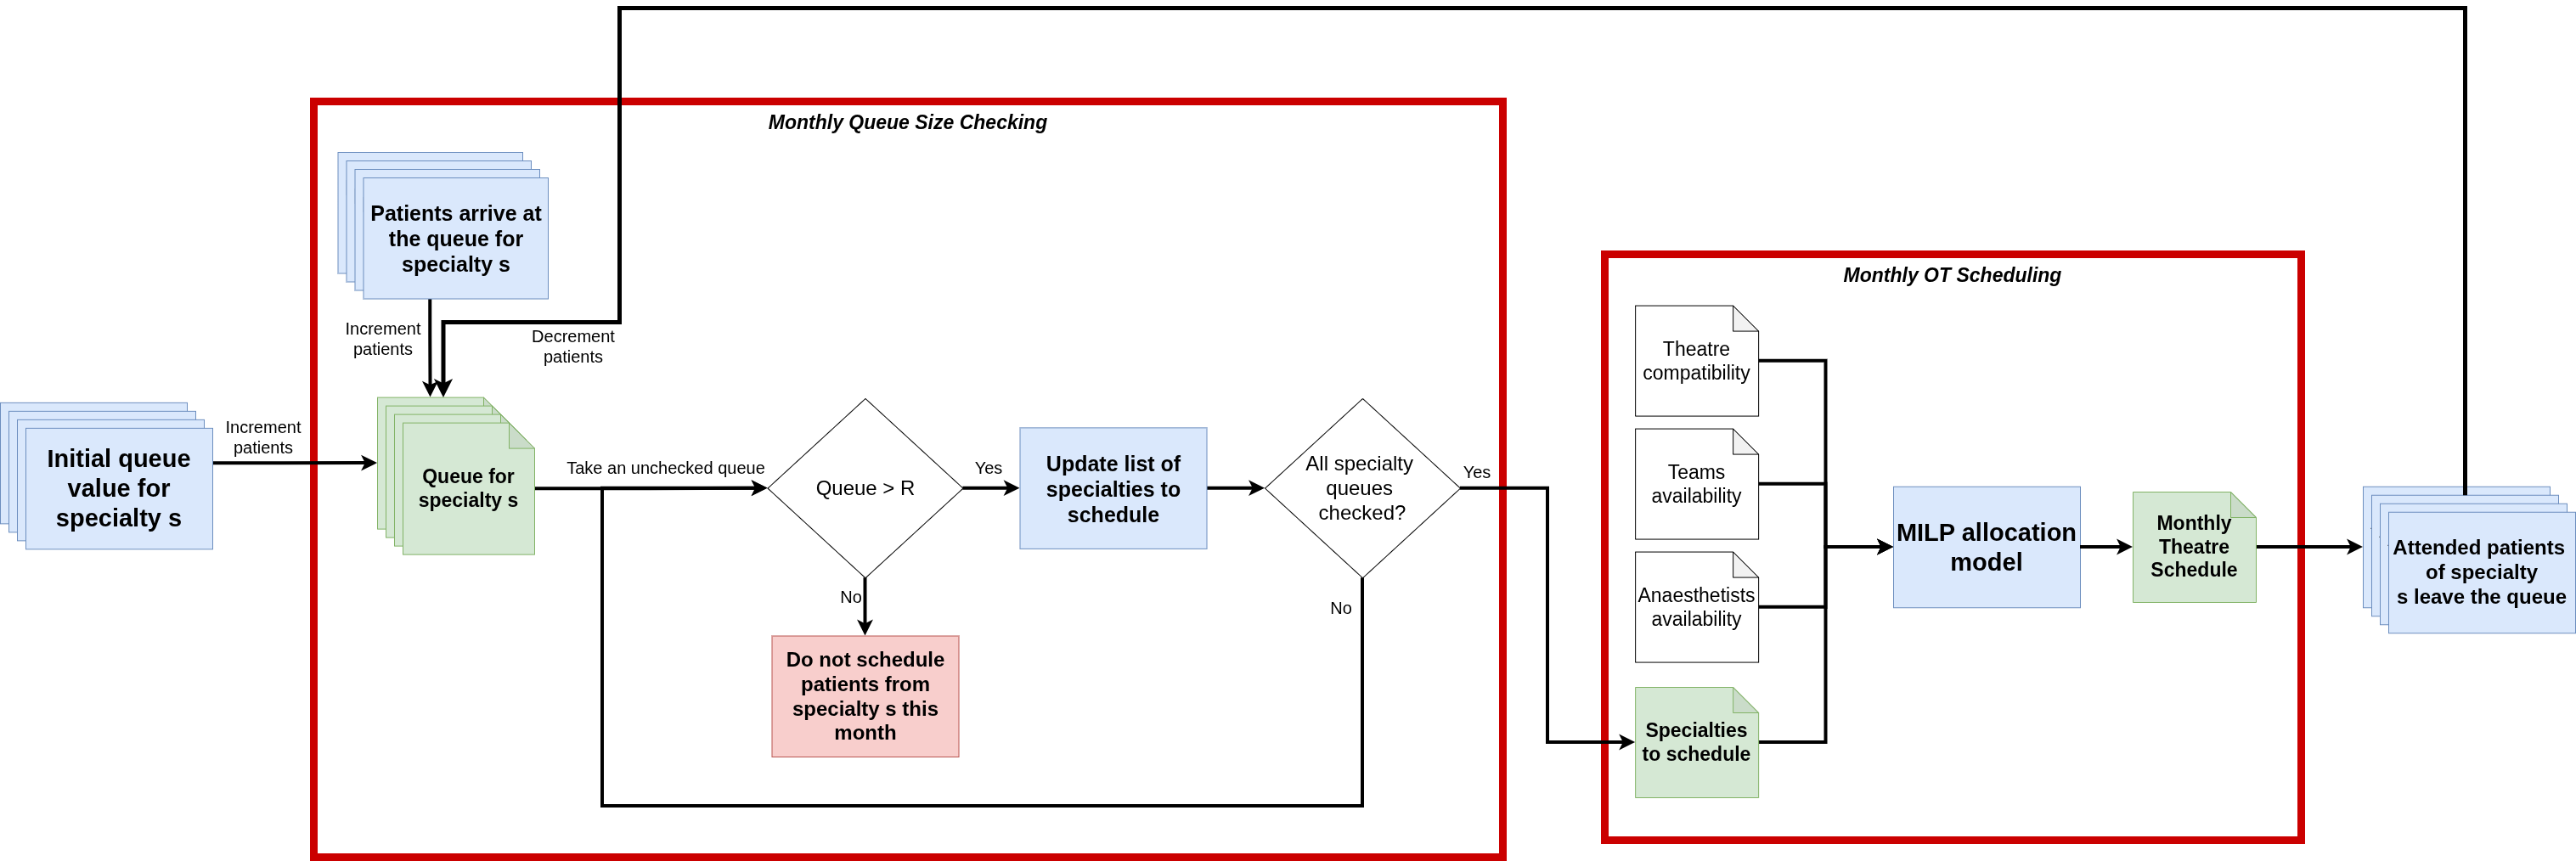
\includegraphics[width=0.9\textwidth]{images/experimental_design.png}
    \caption{Long-term simulation flow.}
    \label{fig:longterm_simulation}
\end{figure}

To assess long-term stability and the baseline, we perform $100$ independent simulation runs each, using different random seeds to capture the stochasticity in surgery durations and patient arrivals.

\subsection{Results from Strategic Decision-Making\label{sec:longterm_analysis}}

\subsubsection{$(R,Q)$ Policy Results}
% apresentar os tamanhos dos Q para cada especialidade (em numero de cirurgias)
% apresentar os tamanhos dos Q para cada especialidade (em numero de blocos)
% analise: quais especialidades tem Q mais altos? quais tem Q mais baixos? qual a relação entre Q e a demanda? qual a relação entre Q e o numero de blocos alocados? qual a relação entre Q e o tempo de espera dos pacientes?


\subsubsection{Overtime and Cancellation Results}
% apresentar resultados do newsvendor: 
% - o valor de t* para cada especialidade (tabela em apendice, talvez?)
% - grafico de distribuições de se planejar k cirurgias
% - analise: quais especialidades tem t* mais altos? quais tem t* mais baixos? talvez(relacao do t* com a distribuição do grafico); analisar o grafico e os impactos: quanto mais cirurgias planejar, maior a chande de cancelar (explicar intuitivamente)
% apresentar resultados do inventory-model:
% - grafico de custo vs ganho (uma ou duas especialidades)
% - analise: como isse modelo foi usado para definir um numero de otimo de cirurigas a planejar? por que ele é bom? qual o impacto do custo de overtime e cancelamento? qual o impacto da forma da função de custo (quadratica)?


\subsection{Long-term Stability Analysis\label{sec:otscheduling}}
In this section, we evaluate the long-term stability of the system under the proposed approach and compare it with the baseline policy.
We analyse the evolution of patient queues over time and the allocation of operating theatre blocks, highlighting the differences between the two approaches.

\subsubsection{Queue Management Results}
The one-year simulation horizon enables the analysis of queue dynamics under both the proposed framework and the baseline policy. 
As results are obtained from $100$ independent runs, we also assess variability through the 10--90\% percentile interval, which provides insight into the robustness of each approach.
\textcolor{red}{percebi que os graficos tem a mesma cor pro baseline e o proposto... todo: corrgir isso}

\begin{figure}[htb]
    \centering
    \begin{subfigure}[b]{0.45\textwidth}
        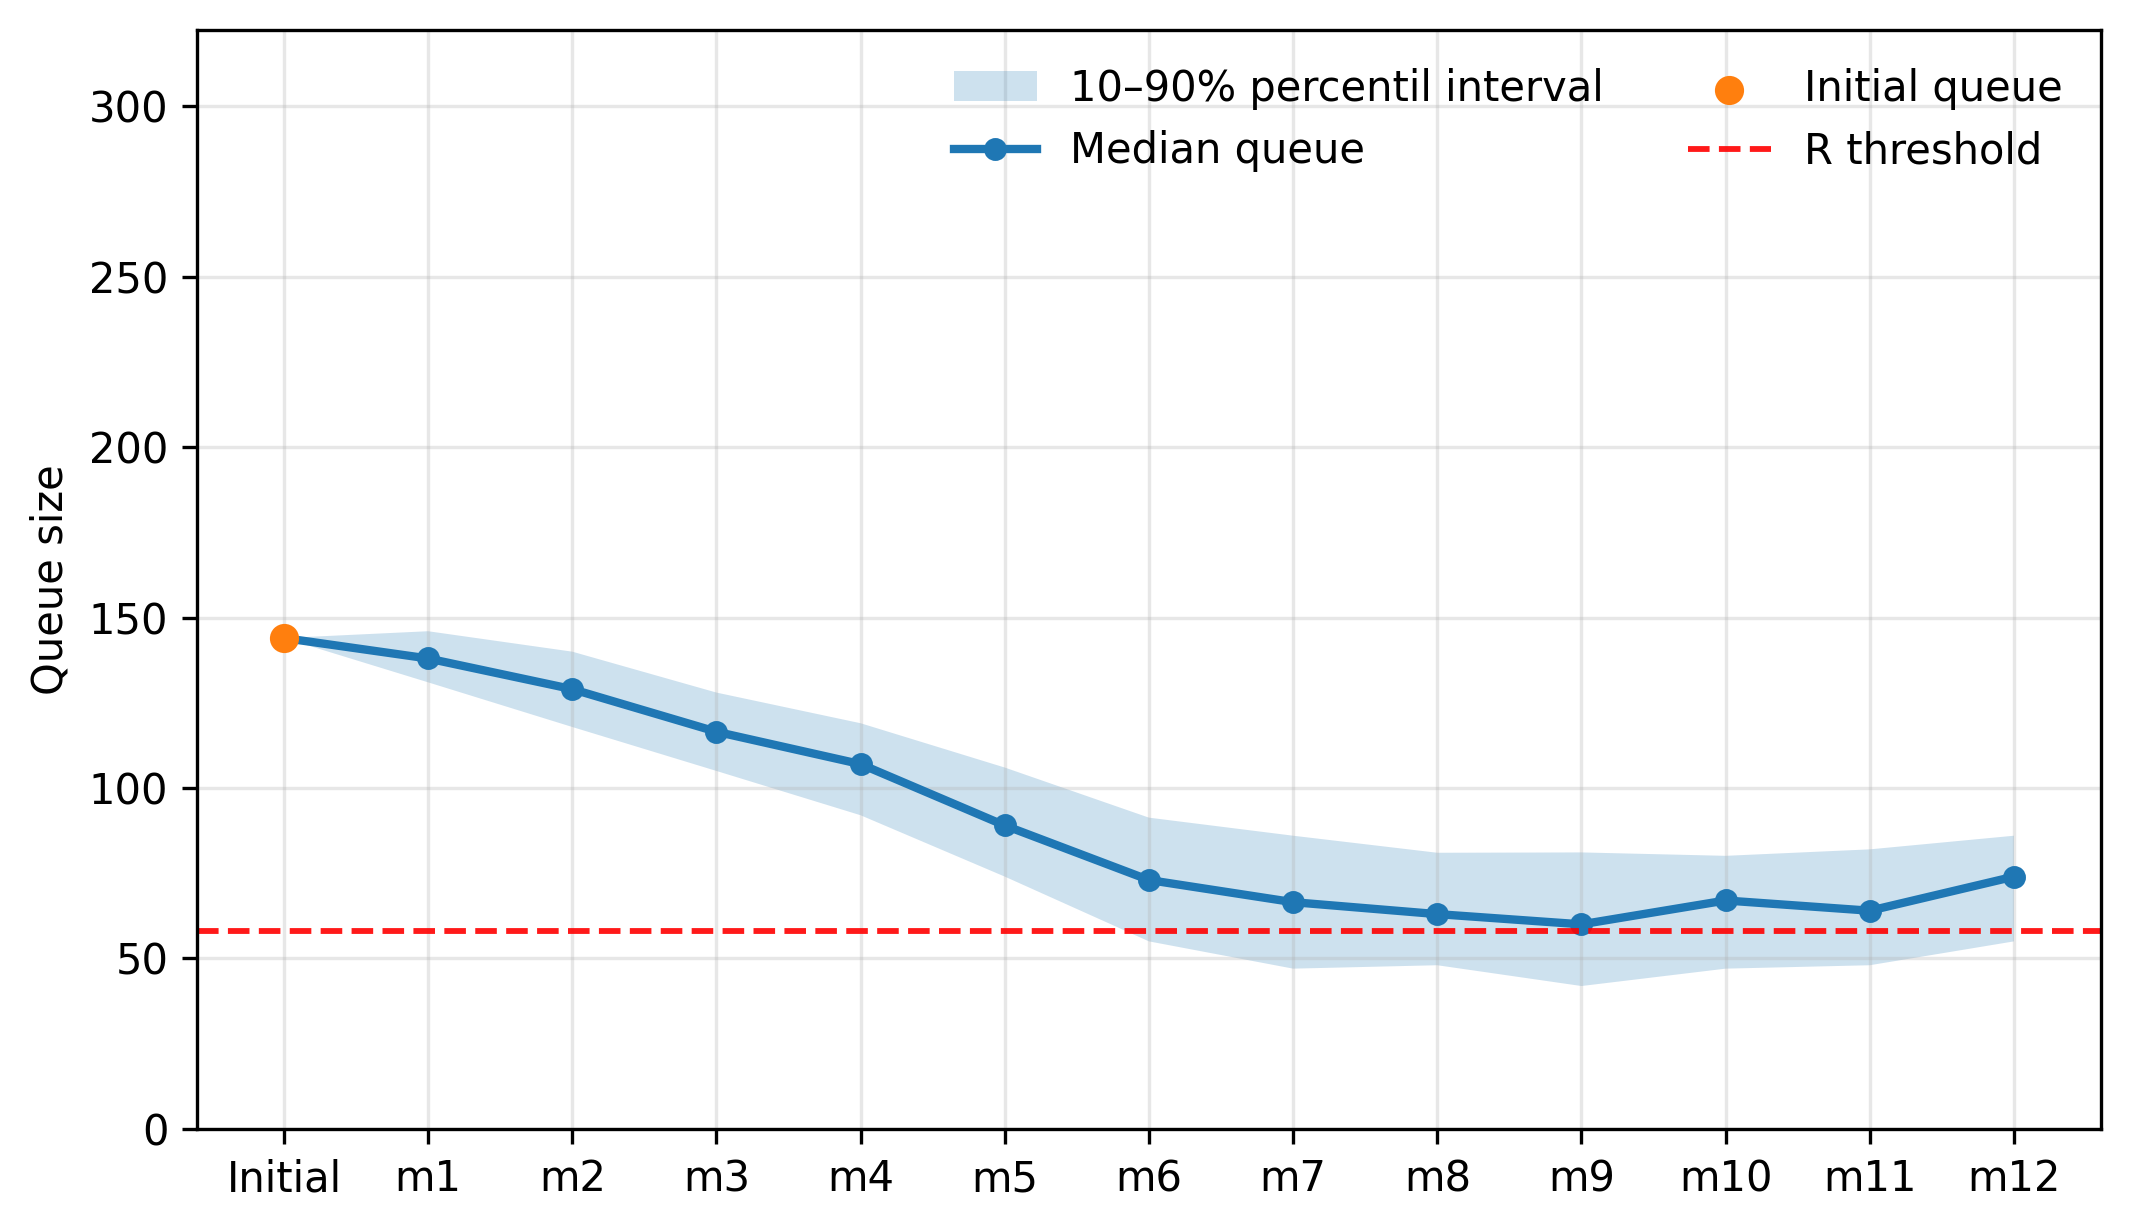
\includegraphics[width=\textwidth]{images/queue_trend_eda_infantil.png}
        \caption{Proposed approach.}
        \label{fig:eda_proposed}
    \end{subfigure}
    \hfill
    \begin{subfigure}[b]{0.45\textwidth}
        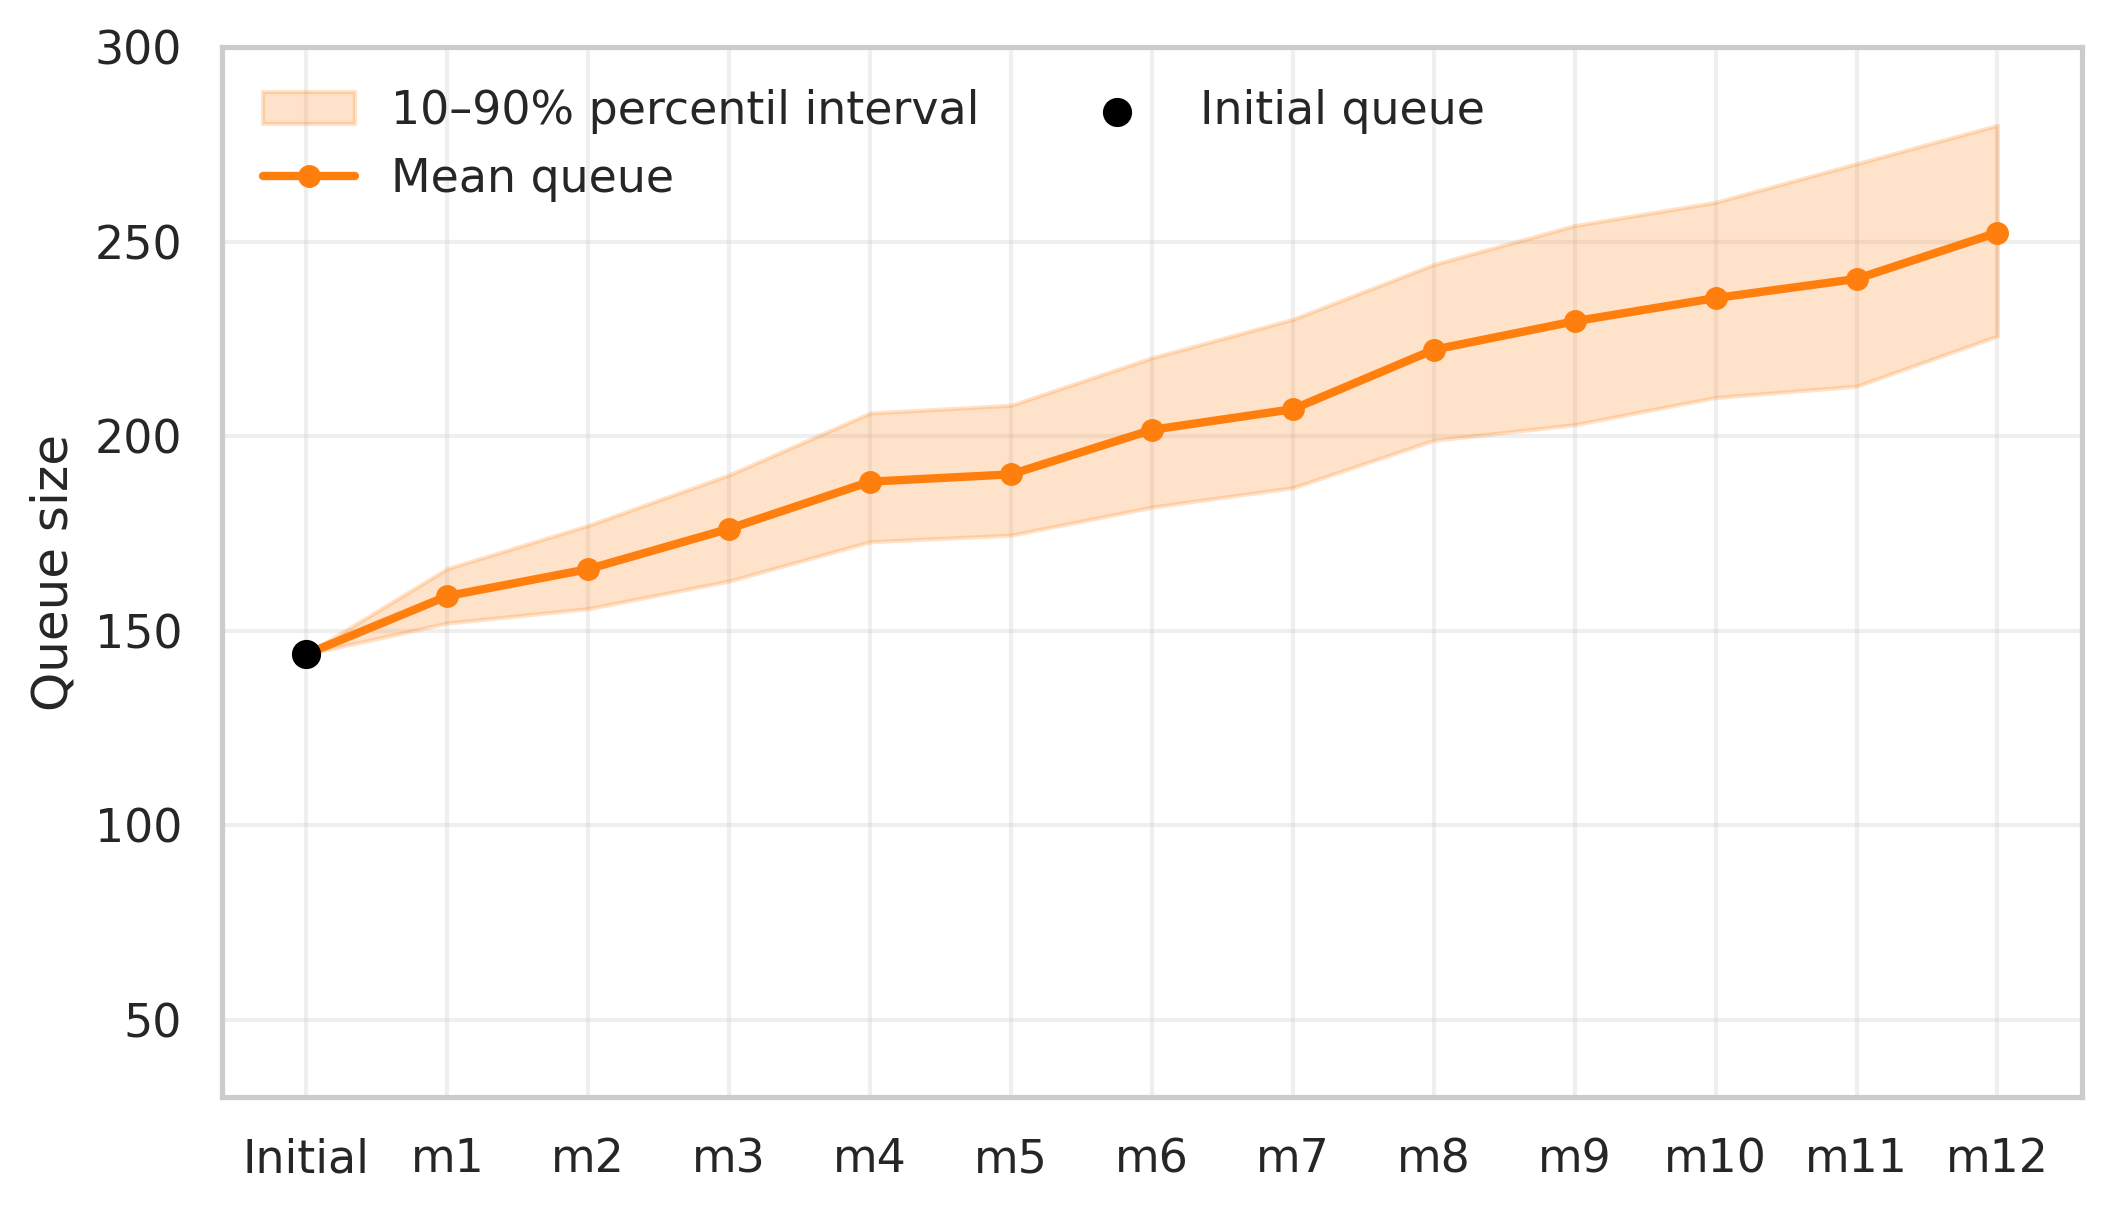
\includegraphics[width=\textwidth]{images/baseline_queue_trend_eda_infantil.png}
        \caption{Baseline policy.}
        \label{fig:eda_baseline}
    \end{subfigure}
    \caption{Evolution of patient queues over time for the subspecialty \textit{UDP -- Pediatric}.}
    \label{fig:queue_evolution_eda}
\end{figure}

Figure~\ref{fig:queue_evolution_eda} illustrates the evolution of the patient queue for the subspecialty \textit{Upper Digestive Endoscopy (UDP) -- Pediatric}. 
Under the proposed approach (Figure~\ref{fig:eda_proposed}), the queue exhibits a clear decreasing trend from the initial level, with variability gradually reducing over time. 
Once the queue approaches the threshold $R$ (around month 6--9), the policy implicitly limits further allocations to this subspecialty, allowing capacity to be redirected to others. 
As a result, the queue stabilises around the target level, avoiding both excessive backlog and unnecessary over-allocation.

In contrast, the baseline policy (Figure~\ref{fig:eda_baseline}) lacks any feedback mechanism based on queue size. 
Although an initial reduction is observed, the queue subsequently increases and displays a persistent upward trend, with widening variability. 
This indicates that the system is unable to regulate demand and capacity effectively, leading to potential instability and longer waiting times.

A similar behaviour is observed for the subspecialty \textit{Gastroenterology -- Esophagus-Stomach-Duodenum (ESD)} in Figure~\ref{fig:queue_evolution_gast_eed}. 
Under the proposed approach (Figure~\ref{fig:gast_proposed}), the queue decreases more rapidly than in the previous case, reflecting the higher service capacity available for this subspecialty. 
The queue then stabilises close to the threshold $R$, again indicating effective balancing between demand and allocation decisions.

\begin{figure}[ht]
    \centering
    \begin{subfigure}[b]{0.45\textwidth}
        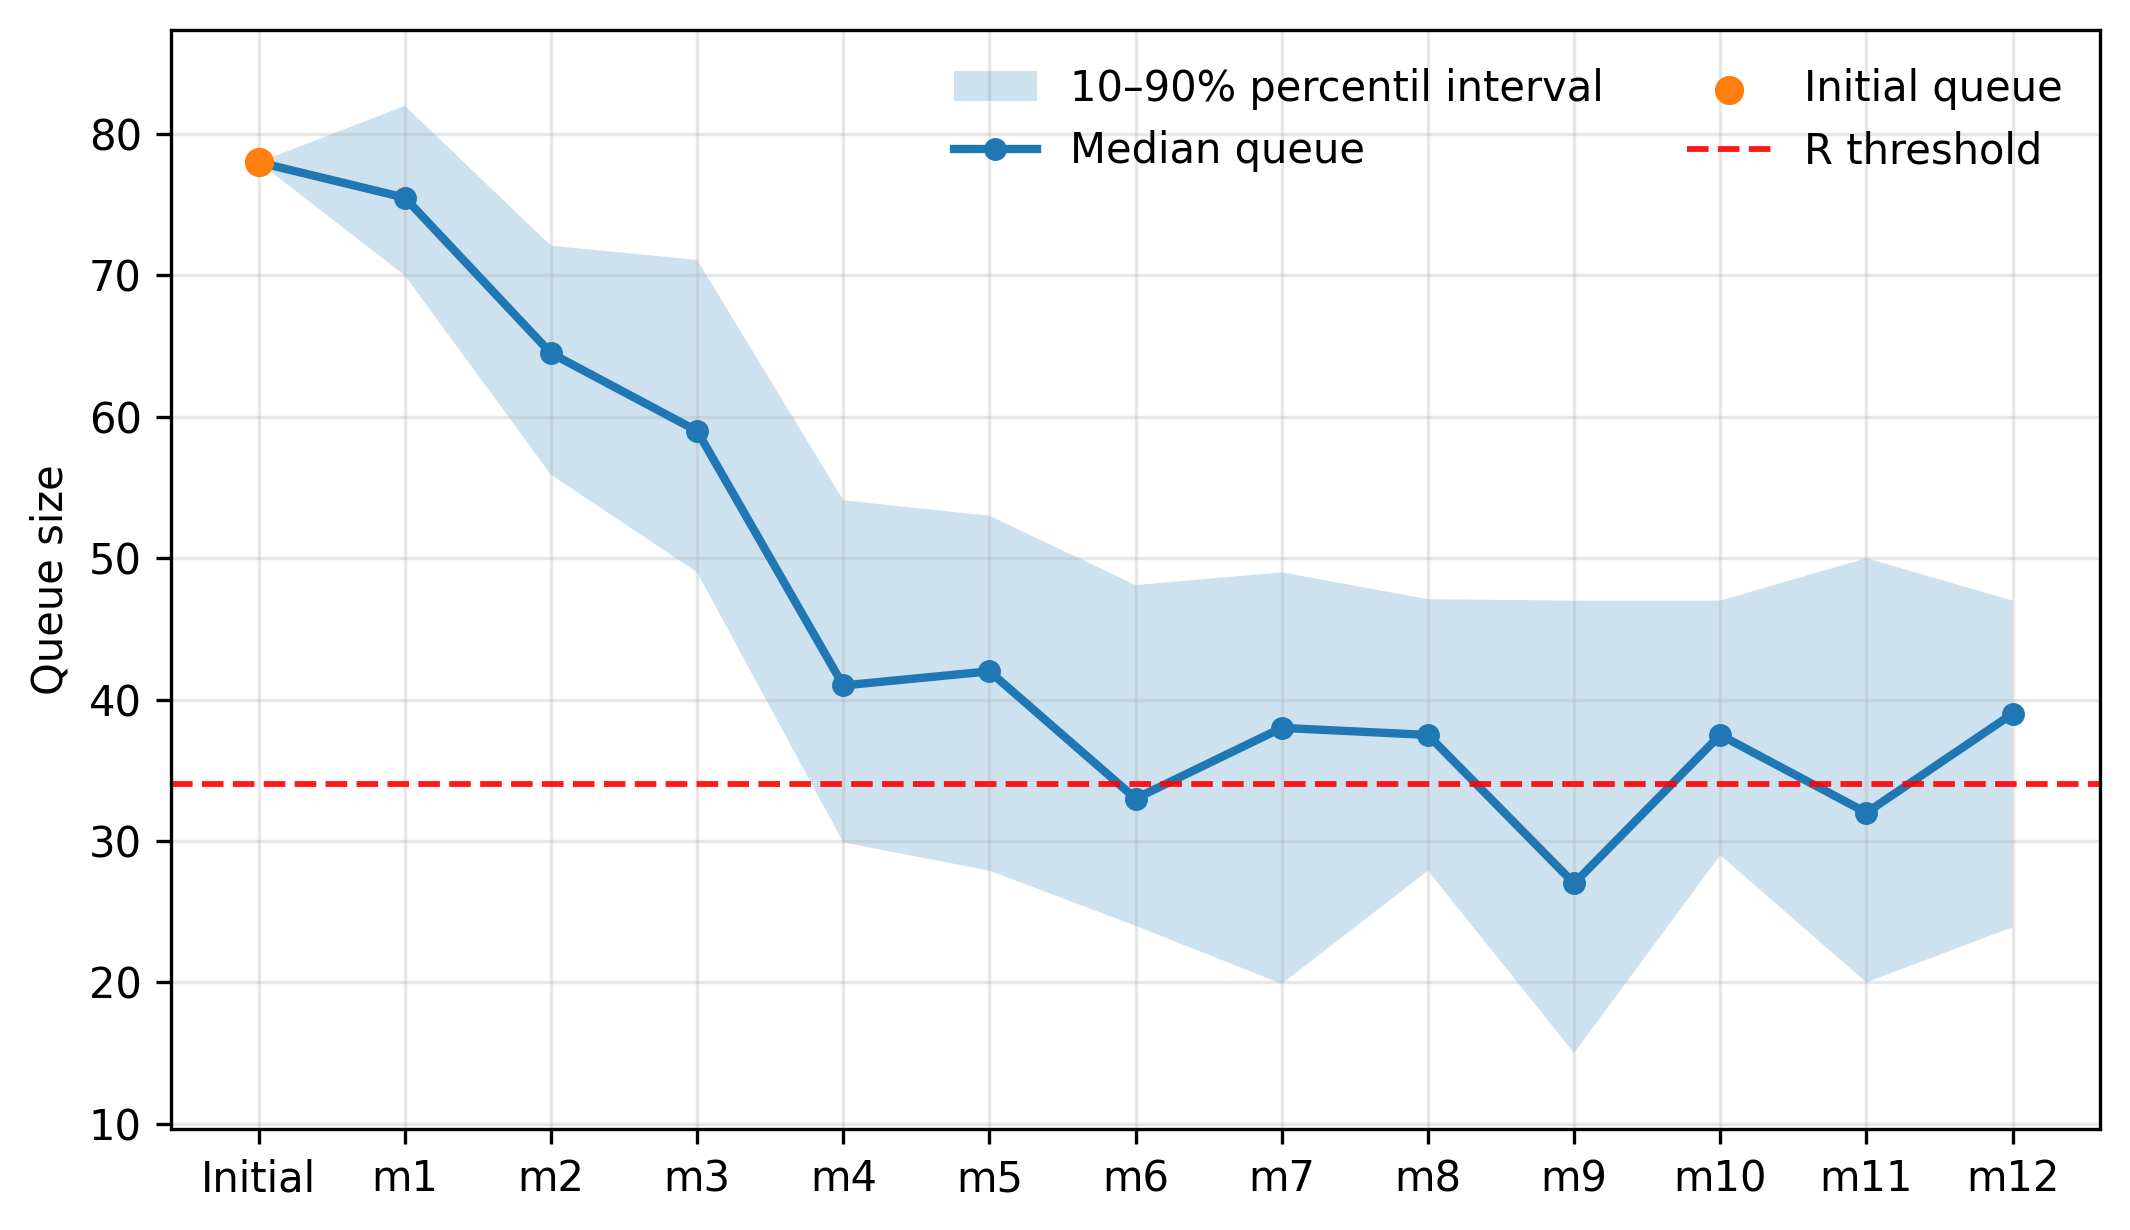
\includegraphics[width=\textwidth]{images/queue_trend_gast_eed.png}
        \caption{Proposed approach.}
        \label{fig:gast_proposed}
    \end{subfigure}
    \hfill
    \begin{subfigure}[b]{0.45\textwidth}
        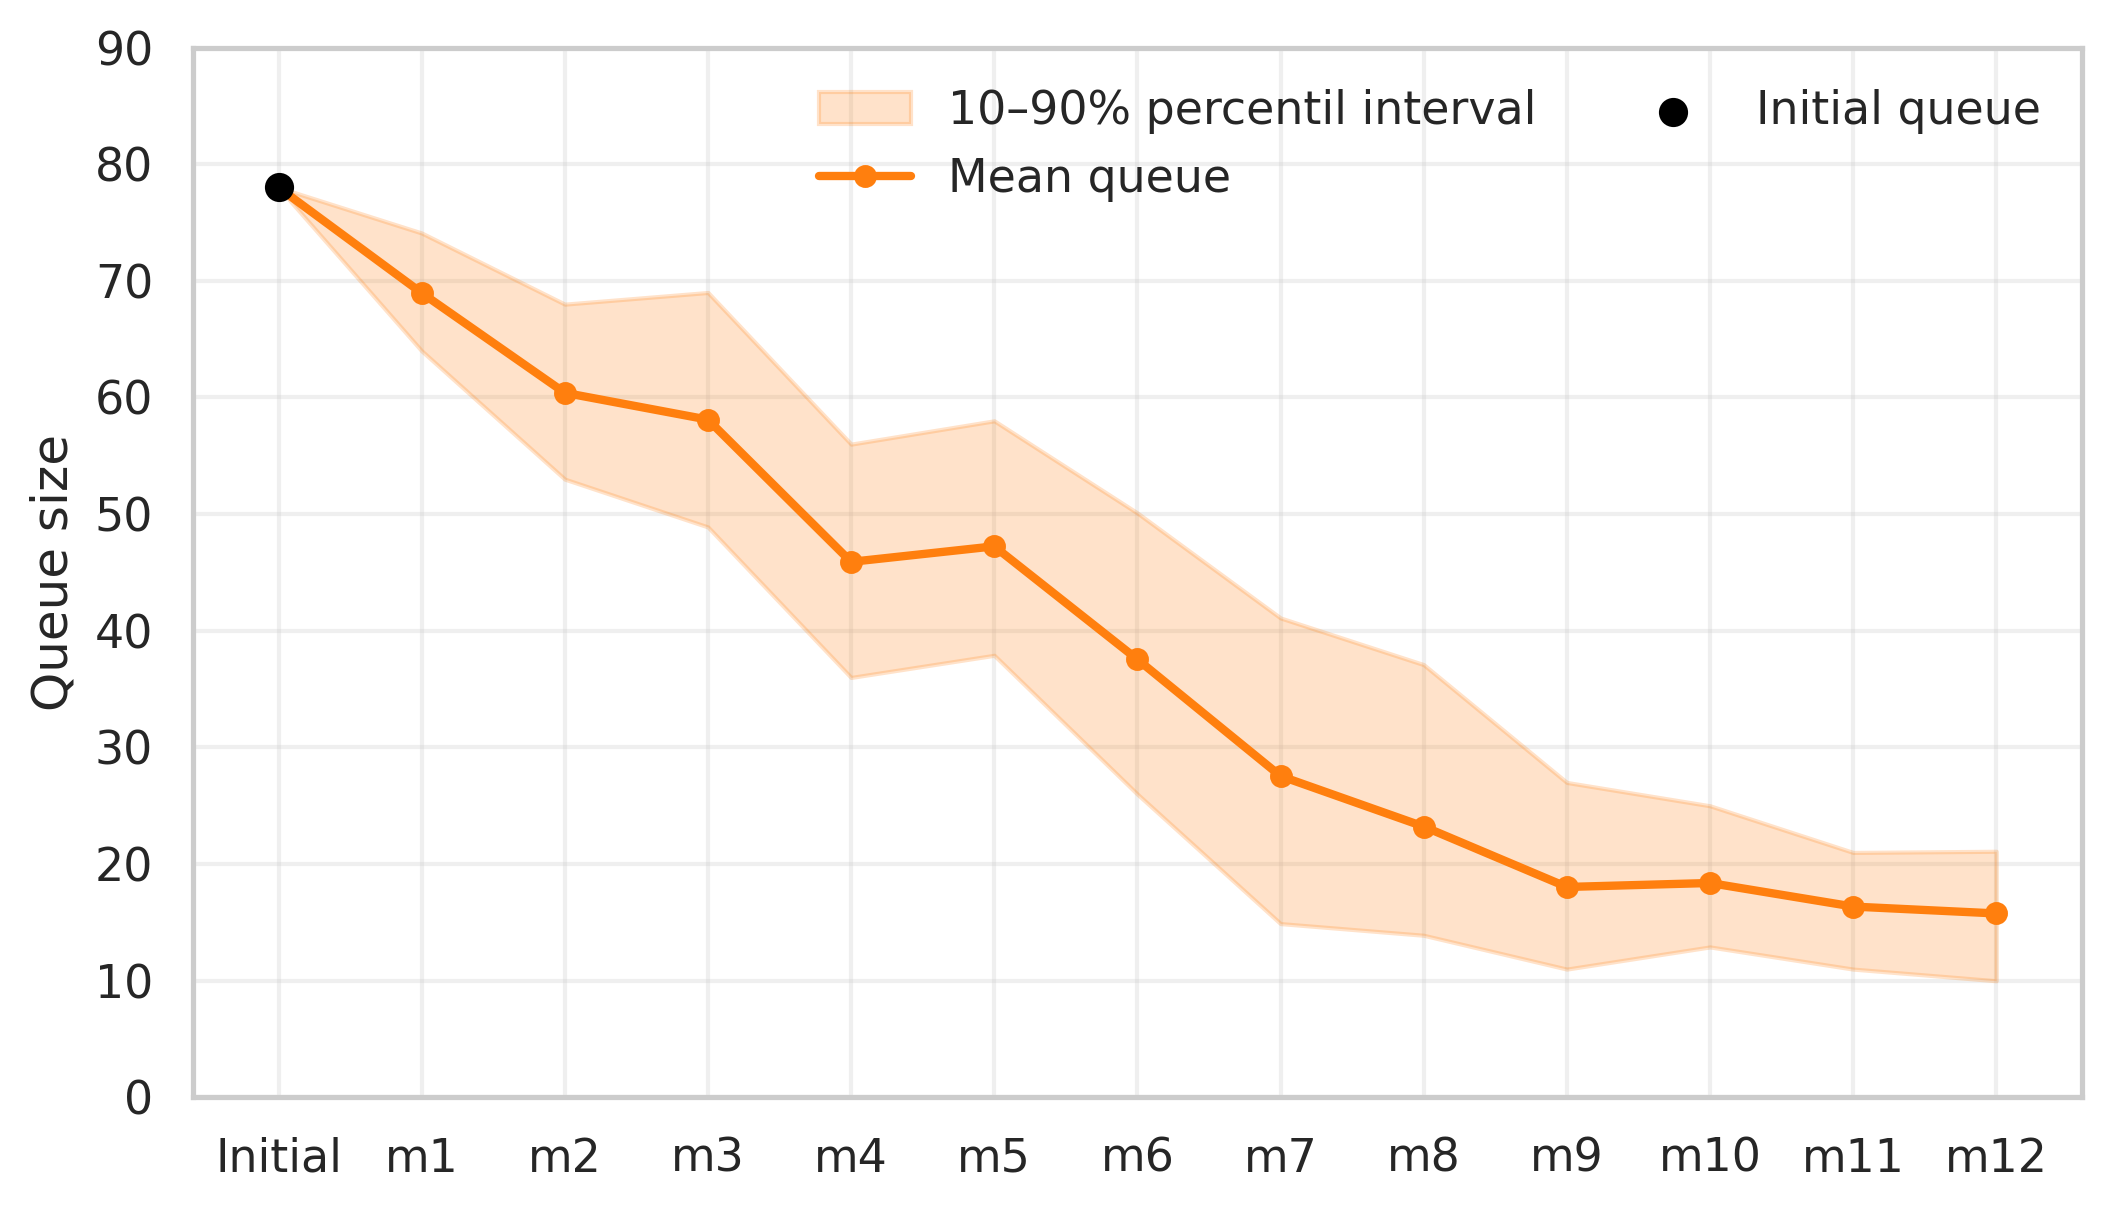
\includegraphics[width=\textwidth]{images/baseline_queue_trend_gast_eed.png}
        \caption{Baseline policy.}
        \label{fig:gast_baseline}
    \end{subfigure}
    \caption{Evolution of patient queues over time for the subspecialty \textit{Gastroenterology -- ESD}.}
    \label{fig:queue_evolution_gast_eed}
\end{figure}

For the baseline policy (Figure~\ref{fig:gast_baseline}), the queue also decreases over time, as this subspecialty is consistently allocated and benefits from sufficient capacity. 
However, this apparent improvement is misleading when viewed at the system level. 
Because the baseline allocates all subspecialties uniformly, without considering their relative queue sizes, it may over-serve some subspecialties (such as ESD) while neglecting others. 
This lack of awareness of queue dynamics can lead to imbalances across the system, even if individual queues appear well behaved.

These results show that the $(R,Q)$-based control introduces a feedback mechanism that regulates queue sizes around a target level, reduces variability, and promotes efficient use of capacity. 
In contrast, the baseline policy operates in an open-loop manner, which may lead to uncontrolled growth or inefficient allocation of resources. 
Detailed results for all subspecialties are provided in Appendix~\ref{app:queue_evolution}.

\subsubsection{OT Allocation Results}
% apresentar o grafico que mostra o quanto o framework alocou quando comparado ao intervalo Q (o grafico que brinquei que é ilícito -- só que melhorado)
% - discutir aqui que nossa abordagem nao aloca todas especialidades todo mes, o que dá vazao pra outras especialidades, aí dá pra mostrar dois graficos desse
% apresentar escalas mensais de alocação de sala

\section{Conclusions and Future Directions\label{sec:conclusion}}

% *******************************************
\bibliographystyle{elsarticle-harv}
\scriptsize{\bibliography{ref}}
% *******************************************
\end{document}

\endinput
%%
%% End of file `elsarticle-template-harv.tex'.


